\documentclass[a4paper,12pt]{article}
\usepackage[polish]{babel}
\usepackage[utf8]{inputenc}
\usepackage[T1]{fontenc}
\usepackage{lmodern}
\usepackage[top=3cm,bottom=2.5cm,left=3cm,right=3cm]{geometry}
\usepackage{graphicx}
\usepackage{url}
\usepackage{amsmath}
\usepackage{amssymb}
\usepackage{float}
\usepackage{enumitem}
\usepackage{listings}
\usepackage{xcolor}
\usepackage{booktabs}    % ładne linie w tabeli
\usepackage{tabularx}    % elastyczne kolumny X
\usepackage{siunitx}  

\lstset{
  language=Python,
  basicstyle=\ttfamily\scriptsize,
  keywordstyle=\color{blue}\bfseries,
  commentstyle=\color{gray}\itshape,
  stringstyle=\color{red},
  showstringspaces=false,
  frame=single,
  breaklines=true,
  literate={ą}{{\k{a}}}1 {ć}{{\'c}}1 {ę}{{\k{e}}}1 {ł}{{\l{}}}1 {ń}{{\'n}}1 {ó}{{\'o}}1 {ś}{{\'s}}1 {ź}{{\'z}}1 {ż}{{\.z}}1
    {Ą}{{\k{A}}}1 {Ć}{{\'C}}1 {Ę}{{\k{E}}}1 {Ł}{{\L{}}}1 {Ń}{{\'N}}1 {Ó}{{\'O}}1 {Ś}{{\'S}}1 {Ź}{{\'Z}}1 {Ż}{{\.Z}}1,
}

\begin{document}
\begin{titlepage}
  \thispagestyle{empty}
  \begin{center}
    % --- GÓRA ---
    {\LARGE\bfseries Sztuczna inteligencja\par}
    \vspace{1.5cm}

    % --- ŚRODEK: podtytuł ---
    {\large Uczenie ze wzmocnieniem:\\
    Projekt i implementacja autonomicznego agenta gry Snake wykorzystującego\\
    Q-learning oraz sieci neuronowe\par}
    \vspace{3cm}

    % --- Autor ---
    {\Large Autor:\\
    Kacper Hyliński\par}
    {\large kierunek Informatyka\par}
    \vfill

    % --- STOPKA ---
    {\large Rzeszów, 2025\par}
    \vspace{0.4cm}
    {\normalsize Wydział Elektrotechniki i Informatyki\par}
    {\normalsize Politechnika Rzeszowska im.\ Ignacego Łukasiewicza\par}
  \end{center}
\end{titlepage}
 
 \clearpage
  \pagenumbering{roman}
  \thispagestyle{empty}
  \tableofcontents
  \clearpage
  \pagenumbering{arabic}

  \section{Cel projektu}
Celem niniejszego projektu jest opracowanie, implementacja oraz porównawcza analiza dwóch metod uczenia ze wzmocnieniem w zmodyfikowanym środowisku gry Snake, w którym agent ponosi karę za kolizję ze ścianami. W pierwszym podejściu zastosowano klasyczny algorytm Q-learning, natomiast w drugim – jego rozszerzenie o głęboką sieć neuronową (Deep Q-Network, DQN).

W ramach projektu zostanie utworzone środowisko symulacyjne, w którym agent będzie zobligowany do identyfikacji kluczowych elementów otoczenia, takich jak obszary zagrożenia oraz źródła pożywienia, a następnie do podejmowania decyzji na podstawie obserwowanych stanów. Ponadto zaimplementowany zostanie wariant Double DQN, a proces uczenia zostanie przyspieszony poprzez integrację technologii CUDA, z zapewnieniem możliwości alternatywnego przeprowadzenia treningu na procesorze centralnym w przypadku braku wsparcia GPU.

Dla optymalizacji przebiegu treningu opracowany zostanie również uproszczony interfejs gry, pozbawiony renderowania graficznego na ekranie, co pozwoli na znaczące zwiększenie efektywności procesu uczenia.
\clearpage  























\section{Część teoretyczna}
\subsection{Model neuronu}
\begin{figure}[h!]
    \centering
    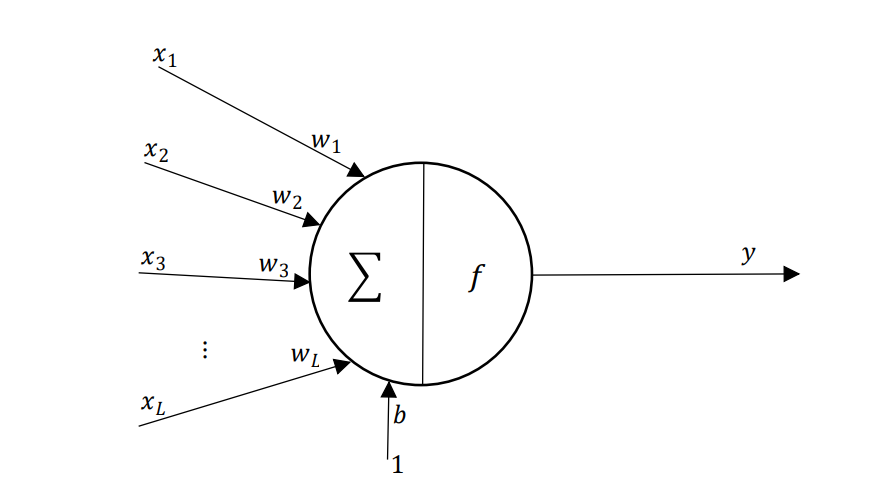
\includegraphics[width=1\linewidth]{image.png}
    \caption{Model Neuronu \cite{RZajdelNeuron}.}
\end{figure}

\noindent $\boldsymbol{x_1 - x_L}$ - sygnał wejściowy, \newline
 $\boldsymbol{w_1 - w_L}$ - współczynnik wagowy, \newline
$\boldsymbol{b}$ - bias, \newline
$\boldsymbol{\sum}$  - sumator, \newline
$\boldsymbol{f}$ - funkcja aktywująca, \newline
$\boldsymbol{y}$ - wartość wyjściowa 
\begin{equation}
y = f\Bigl(\sum_{j=1}^{L} w_j\,\cdot x_j + b\Bigr)
\end{equation}
Symbol \(x_j\) oznacza \(j\)-ty sygnał wejściowy (\(j = 1, 2, \dots, L\)), natomiast \(w_j\) odpowiada przypisanej mu wadze.

\medskip

Sumę ważoną sygnałów wejściowych wraz z wartością przesunięcia (biasu) określa się mianem \textit{łącznego pobudzenia neuronu}, które w dalszej części oznaczane będzie symbolem \(z\):
\begin{equation}
z = \sum_{j=1}^{L} w_j \cdot x_j + b.
\end{equation}


\subsection{Sieć neuronowa wielowarstwowa (MLP)}

\begin{figure}[h!]
    \centering
    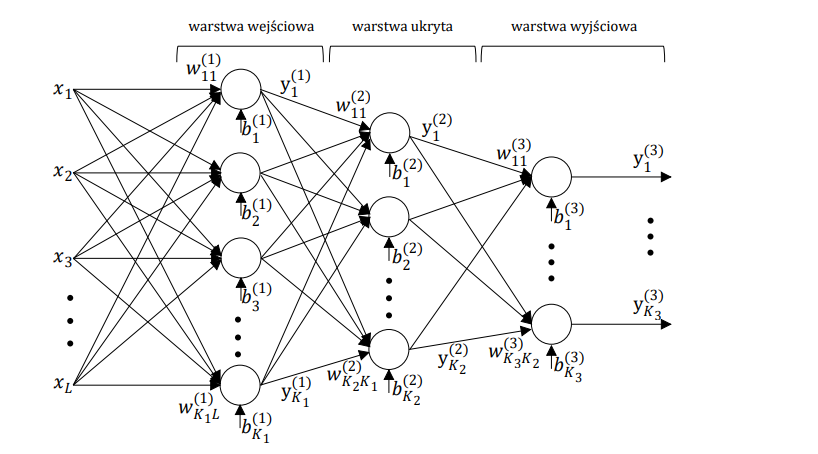
\includegraphics[width=1\linewidth]{MLP.png}
    \caption{Sieć jednokierunkowa wielowarstwowa \cite{RZajdelMLP}.}
\end{figure}

Taką sieć nazywa się trójwarstwową. Występują tu połączenia pomiędzy warstwami neuronów typu każdy z każdym.  
Sygnały wejściowe podawane są do warstwy wejściowej neuronów, których wyjścia stanowią sygnały źródłowe dla kolejnej warstwy.  
Można wykazać, że sieć trójwarstwowa nieliniowa jest w stanie odwzorować praktycznie dowolne odwzorowanie nieliniowe.

Każda warstwa neuronów posiada swoją macierz wag \(\mathbf{w}\), wektor przesunięć \(\mathbf{b}\), funkcję aktywacji \(f\) i wektor sygnałów wyjściowych \(\mathbf{y}\).  
Aby je rozróżniać w dalszych rozważaniach, do każdej z wielkości dodano numer warstwy, której dotyczą.  
Na przykład dla warstwy drugiej (ukrytej) macierz wag oznaczana będzie symbolem \(\mathbf{w}^{(2)}\).  
Działanie każdej z warstw można rozpatrywać oddzielnie.  
I tak np. warstwa druga posiada: \(L = K_1\) sygnałów wejściowych, \(K = K_2\) neuronów i macierz wag \(\mathbf{w} = \mathbf{w}^{(2)}\) o rozmiarach \(K_2 \times K_1\).  
Wejściem warstwy drugiej jest wyjście warstwy pierwszej \(\mathbf{x} = \mathbf{y}^{(1)}\), a wyjściem \(\mathbf{y} = \mathbf{y}^{(2)}\).  
Działanie poszczególnych warstw dane jest przez

\begin{equation}
y^{(1)} = f^{(1)}\left(w^{(1)}x + b^{(1)}\right), 
\end{equation}
\begin{equation}
y^{(2)} = f^{(2)}\left(w^{(2)}y^{(1)} + b^{(2)}\right), 
\end{equation}
\begin{equation}
y^{(3)} = f^{(3)}\left(w^{(3)}y^{(2)} + b^{(3)}\right).
\end{equation} 

Działanie całej sieci można więc opisać jako
\begin{equation}
\mathbf{y}^{(3)} = f^{(3)}\left( \mathbf{w}^{(3)} f^{(2)}\left( \mathbf{w}^{(2)} f^{(1)}\left( \mathbf{w}^{(1)} \mathbf{x} + \mathbf{b}^{(1)} \right) + \mathbf{b}^{(2)} \right) + \mathbf{b}^{(3)} \right).
\end{equation}

\cite{RZajdelMLP}



W projekcie Snake AI do aproksymacji funkcji wartości $Q(s,a)$ wykorzystujemy wielowarstwową sieć neuronową (MLP) o strukturze:

\begin{itemize}
\item Warstwa wejściowa: wymiar wektora stanu $d=11$ cech,
\item trzy warstwy ukryte:
\begin{itemize}
\item pierwsza z $H_1=256$ neuronów,
\item druga z $H_2=256$ neuronów,
\item trzecia z $H_3 = 128$ neuronów,
\end{itemize}
\item Warstwa wyjściowa: liczba wyjść równa liczbie akcji $|A|=3$.
\end{itemize}

\subsection{MLP w projekcie Snake AI}
W projekcie Snake AI do aproksymacji funkcji wartości Q(s,a) wykorzystujemy wielowarstwową sieć neuronową (MLP) składającą się z warstwy wejściowej, dwóch warstw ukrytych i warstwy wyjściowej. 

\begin{equation}
\mathbf{y}^{1} = f^{1}(\mathbf{z}^{1}) = f^{1}(\mathbf{w}^{1} \mathbf{x} + \mathbf{b}^{1}) 
\end{equation}
\begin{equation}
\mathbf{y}^{2} = f^{2}(\mathbf{z}^{2}) = f^{2}(\mathbf{w}^{2} \mathbf{y}^{1} + \mathbf{b}^{2}) 
\end{equation}
\begin{equation}
\mathbf{y}^{3} = f^{3}(\mathbf{z}^{3}) = f^{3}(\mathbf{w}^{3} \mathbf{y}^{2} + \mathbf{b}^{3}) 
\end{equation}
\begin{equation}
\mathbf{y}^{4} = f^{4}(\mathbf{z}^{4}) = f^{4}(\mathbf{w}^{4} \mathbf{y}^{3} + \mathbf{b}^{4})
\end{equation}

Gdzie \(f^{1}, f^{2}, f^{3}\) to funkcje Leaky ReLU, a \(f^{4}\) to funkcja liniowa.

\textit{wzór opisujący działanie całej sieci jako złożenie funkcji:}

\begin{equation}
\mathbf{y}^{4} = f^{4}\left( \mathbf{w}^{4} f^{3} \left( \mathbf{w}^{3} f^{2} \left( \mathbf{w}^{2} f^{1}(\mathbf{w}^{1} \mathbf{x} + \mathbf{b}^{1}) + \mathbf{b}^{2} \right) + \mathbf{b}^{3} \right) + \mathbf{b}^{4} \right)
\end{equation}

\subsection{Funkcje aktywacji}

W ramach niniejszego projektu, którego celem jest implementacja agenta Deep Q-Network (DQN) w środowisku gry Snake, zastosowano różne funkcje aktywacji. Ich dobór został przeprowadzony w sposób celowy i dostosowany do charakterystyki poszczególnych warstw sieci neuronowej.

\textbf{Leaky ReLU} – funkcja aktywacji, która wprowadza niewielki współczynnik nachylenia dla wartości ujemnych, co pozwala na uniknięcie problemu zanikania gradientu i „martwych neuronów”. Funkcja ta jest zdefiniowana jako:
\begin{equation}
f(x) = \begin{cases}
x & \text{jeśli } x > 0 \\
\alpha x & \text{jeśli } x \leq 0
\end{cases}
\end{equation}

lub w bardziej zwartej postaci:

\begin{equation}
f(x) = \max(\alpha x, x),
\end{equation}

gdzie \(\alpha\) to mała wartość (w naszym projekcie \(0{,}01\)), która kontroluje nachylenie dla wartości ujemnych. W sieci DQN używamy Leaky ReLU we wszystkich warstwach ukrytych.

\medskip

\textbf{Funkcja liniowa} – funkcja aktywacji używana w warstwie wyjściowej sieci DQN, która nie wprowadza żadnej nieliniowości, co pozwala na nieograniczony zakres wartości wyjściowych. Jest zdefiniowana jako:
\begin{equation}
f(x) = x
\end{equation}

Funkcja ta jest szczególnie przydatna w warstwie wyjściowej sieci aproksymującej funkcję \(Q\), gdzie wyjścia mogą przyjmować dowolne wartości rzeczywiste.

\begin{figure}[H]
    \centering
    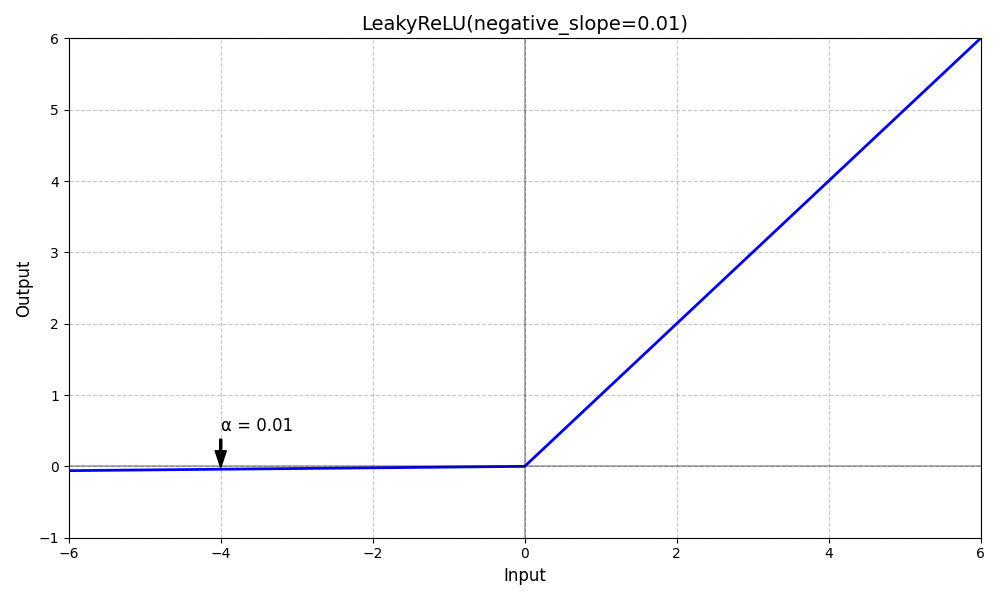
\includegraphics[width=1\linewidth]{LeakyRelu.png}
    \caption{Wykres LeakyRelu}
\end{figure}

Funkcja liniowa w warstwie wyjściowej sieci DQN została wybrana ze względu na następujące właściwości i zalety:

\begin{enumerate}[label=\textbf{\arabic*.}, leftmargin=1.5cm]
    \item \textbf{Nieograniczony zakres wartości wyjściowych} – w kontekście aproksymacji funkcji wartości \(Q\), wyjścia sieci mogą przyjmować dowolne wartości rzeczywiste. Funkcja liniowa nie wprowadza żadnych ograniczeń zakresu wartości wyjściowych, co jest kluczowe dla poprawnego przewidywania wartości funkcji \(Q\).

    \item \textbf{Zgodność z teorią DQN} – w oryginalnej publikacji opisującej algorytm Deep Q-Network autorstwa Mnih et al. (2015), również zastosowano liniową funkcję aktywacji w warstwie wyjściowej, co potwierdza zasadność wyboru tego rozwiązania.

    \item \textbf{Rozwiązanie problemu "umierających neuronów":} Standardowa funkcja ReLU zwraca 0 dla wszystkich wartości ujemnych, co może prowadzić do "umierania neuronów", kiedy neuron zawsze daje wartość 0 na wyjściu. LeakyReLU rozwiązuje ten problem, pozwalając na przepływ małego gradientu dla wartości ujemnych.
\end{enumerate}

\clearpage 

\subsection{Wprowadzenie do uczenia ze wzmocnieniem i MDP}
Uczenie ze wzmocnieniem (ang.\ \emph{Reinforcement Learning}, RL) to rodzaj uczenia maszynowego, w którym agent uczy się podejmować sekwencje decyzji poprzez interakcję ze środowiskiem. Po każdej akcji podjętej w stanie środowiska agent otrzymuje \emph{nagrodę} – skalarny feedback – i przechodzi do nowego stanu. Celem agenta jest opracowanie \emph{strategii (polityki)} wyboru akcji maksymalizującej skumulowaną nagrodę w długim horyzoncie czasowym.

Formalnie środowisko modeluje się jako \emph{proces decyzyjny Markowa} (MDP), zdefiniowany jako krotka
\begin{equation}
\mathcal{M} = (\mathcal{S}, \mathcal{A}, P, R),
\end{equation}

gdzie:
\begin{itemize}
  \item $\mathcal{S}$ – zbiór stanów,
  \item $\mathcal{A}$ – zbiór akcji,
  \item $P: \mathcal{S}\times\mathcal{A}\times\mathcal{S}\to[0,1]$, \quad
        $P(s' \mid s,a)=\Pr(s_{t+1}=s'\mid s_t=s,\,a_t=a)$ – funkcja przejścia definiująca rozkład prawdopodobieństwa kolejnego stanu,
  \item $R: \mathcal{S}\times\mathcal{A}\to\mathbb{R}$, \quad
        $R(s,a)=\mathbb{E}[r_{t+1}\mid s_t=s,\,a_t=a]$ – funkcja nagród.
\end{itemize}

Jeśli w chwili $t$ agent znajduje się w stanie $s_t$ i wybierze akcję $a_t$, to z prawdopodobieństwem 
$P(s_{t+1}=s'\mid s_t,a_t)$ przejdzie do stanu $s_{t+1}=s'$ i otrzyma nagrodę 
$r_{t+1}=R(s_t,a_t)$. Proces ten powtarza się iteracyjnie, tworząc ścieżkę stanów, akcji i nagród. 
Sumaryczna zdyskontowana nagroda od chwili $t$ jest zwykle definiowana jako
\begin{equation}
R_t \;=\; \sum_{k=0}^{\infty} \gamma^k\,r_{t+k+1},
\end{equation}
gdzie $\gamma\in[0,1]$ to współczynnik dyskontowania.

gdzie \(0 \le \gamma < 1\) to współczynnik dyskontowania określający ważność przyszłych nagród.\footnote{Niższa wartość \(\gamma\) sprawia, że agent przywiązuje większą wagę do nagród natychmiastowych niż odległych w czasie.} Formalnym celem uczenia ze wzmocnieniem jest znalezienie strategii \(\pi^*\), która maksymalizuje wartość oczekiwaną powyższej sumy nagród.

\subsection*{Funkcja wartości}
Kluczową koncepcją w uczeniu ze wzmocznieniem jest \emph{funkcja wartości}. Dla danej strategii \(\pi\) definiujemy wartość stanu
\begin{equation}
V^{\pi}(s)
= \mathbb{E}\Bigl[\sum_{k=0}^\infty \gamma^k\,r_{t+k+1}\;\Bigm|\;s_t=s\Bigr].
\end{equation}
Analogicznie \emph{funkcję wartości akcji} określa się jako
\begin{equation}
Q^{\pi}(s,a)
= \mathbb{E}\bigl[r_{t+1} + \gamma\,Q^{\pi}\bigl(s_{t+1},\pi(s_{t+1})\bigr)\;\bigm|\;s_t=s,\,a_t=a\bigr].
\end{equation}
Równanie to (zwane \emph{równaniem Bellmana} dla \(Q^\pi\)) wyraża zależność wartości akcji od natychmiastowej nagrody oraz wartości przyszłego stanu. 

Dla strategii optymalnej \(\pi^*\), maksymalizującej zdyskontowaną nagrodę, zachodzi \emph{równanie optymalności Bellmana}:
\begin{equation}
Q^*(s,a)
= r(s,a) + \gamma \sum_{s'} P(s'\mid s,a)\,\max_{a'} Q^*(s',a').
\end{equation}

gdzie \(Q^*(s,a)\) oznacza optymalną funkcję wartości akcji. Innymi słowy, zakładając znajomość pełnego modelu środowiska \((P,R)\), \(Q^*\) spełnia układ równań, z którego (przynajmniej teoretycznie) da się wyznaczyć optymalne wartości i strategię:
\begin{equation}
\pi^*(s) \;=\; \arg\max_{a} Q^*(s,a).
\end{equation}
W praktyce jednak model środowiska często nie jest znany lub zbyt złożony, a przestrzeń stanów ogromna, dlatego stosujemy metody iteracyjne i przybliżone, aby oszacować \(Q^*\).

\subsection{Klasyczny algorytm Q-learning}

Q-learning jest jedną z najpopularniejszych metod uczenia ze wzmocnieniem typu \emph{off-policy} wykorzystujących różnice czasowe. Algorytm ten potrafi uczyć się bezpośrednio na podstawie doświadczeń z interakcji, nie znając apriori funkcji przejścia ani nagród. Zbieżność Q-learningu do optymalnych wartości~$Q^*$ została udowodniona w przypadku dyskretnych przestrzeni stanów i akcji przy odpowiednich założeniach (m.in.\ że każda para stan–akcja jest odwiedzana nieskończenie często, a współczynnik uczenia maleje w czasie).

Algorytm utrzymuje estymację funkcji wartości akcji~$Q(s,a)$ w postaci tabelarycznej (tablicy wartości dla każdej pary stan–akcja). Początkowo przypisuje się jej pewne wartości (np.\ losowe lub zerowe). Następnie agent rozgrywa serię epizodów interakcji ze środowiskiem. W każdym kroku epizodu ze stanu~$s_t$ wybierana jest akcja~$a_t$ zgodnie z aktualną strategią eksploracyjno–eksploatacyjną. Najczęściej stosuje się strategię~$\varepsilon$-greedy, w której z prawdopodobieństwem~$1-\varepsilon$ wybierana jest akcja optymalna według bieżących wartości~$Q$, a z prawdopodobieństwem~$\varepsilon$ agent eksploruje, wybierając akcję losową. Pozwala to uniknąć „uwięzienia” w polityce zachłannej opartej na niedokładnych wartościach i zapewnia odwiedzanie różnych stanów. Parametr~$\varepsilon$ (np.\ początkowo~1) często zmniejsza się w miarę uczenia, aby eksploracja malała z czasem na rzecz eksploatacji zdobytej wiedzy.

Po podjęciu akcji~$a_t$ w stanie~$s_t$ i otrzymaniu nagrody~$r_t$ oraz obserwacji nowego stanu~$s_{t+1}$ następuje aktualizacja oceny $Q(s_t,a_t)$. Klasyczny Q-learning wykorzystuje w tym celu błąd przewidywania, tzw.\ błąd TD (temporal difference), definiowany jako:
\begin{equation}
\delta = r + \gamma \max_{a'} Q(s',a') \;-\; Q(s,a).
\end{equation}

Błąd TD wyraża różnicę między aktualną estymacją wartości \(Q(s,a)\) a wartością docelową
\begin{equation}
y = r + \gamma \max_{a'} Q(s',a'),
\end{equation}
opartą na bieżących ocenach stanu następnego. Następnie wartość \(Q(s,a)\) jest przesuwana w kierunku wartości docelowej o krok proporcjonalny do współczynnika uczenia \(\alpha\) (zwykle \(\alpha \in [0,1]\)):
\begin{equation}
Q(s,a) \;\leftarrow\; Q(s,a) + \alpha\bigl[r + \gamma \max_{a'} Q(s',a') \;-\; Q(s,a)\bigr].
\end{equation}
Powyższa reguła aktualizacji jest implementacją iteracji Bellmana na podstawie pojedynczych doświadczeń. Intuicyjnie, jeśli zaobserwowana natychmiastowa nagroda \(r\) wraz z najlepszą przewidywaną wartością przyszłą \(\max_{a'} Q(s',a')\) przewyższa dotychczasową ocenę \(Q(s,a)\), to \(Q(s,a)\) zostanie zwiększone (i odwrotnie – przeszacowane wartości są zmniejszane). Współczynnik \(\alpha\) reguluje szybkość uczenia: małe \(\alpha\) sprawia, że wartości zmieniają się wolniej (co uśrednia wiele doświadczeń), natomiast \(\alpha = 1\) oznacza całkowite zastąpienie starej wartości nowym jednorazowym oszacowaniem. Dzięki niezależności aktualizacji od konkretnej strategii wyboru akcji (algorytm off-policy), Q-learning w teorii konwerguje do \(Q^*\) nawet jeśli podczas uczenia agent nie zawsze podąża strategią zachłanną.

Algorytm Q-learning stopniowo poprawia przybliżenia wartości akcji. Z czasem, gdy \(Q(s,a)\) zbliża się do wartości optymalnych, strategia zachłanna względem tych wartości staje się strategią optymalną \(\pi^*\). W praktyce tablicowy Q-learning jest stosowany tylko dla stosunkowo niewielkich i dyskretnych przestrzeni stanów, ponieważ przechowywanie i aktualizacja tablicy \(Q(s,a)\) w większych problemach (np.\ gdy stanem jest obraz Atari) jest niewykonalne. Rozwiązaniem problemu skalowalności jest zastąpienie tablicy \(Q\) funkcją przybliżającą – tu z pomocą przychodzi sieć neuronowa\(^*\).

\subsection{Deep Q-Network (DQN)}

Deep Q-Network (DQN) to algorytm, który łączy klasyczny Q-learning z możliwościami głębokich sieci neuronowych do aproksymacji funkcji wartości \(Q\). Fundamentalna koncepcja polega na zastąpieniu tablicy \(Q(s,a)\) przez sieć neuronową \(Q(s,a;\theta)\) parametryzowaną wektorem \(\theta\). Sieć przyjmuje na wejściu reprezentację stanu \(s\) i generuje na wyjściu estymowane wartości \(Q(s,a)\) dla zbioru dostępnych akcji. Dzięki temu podejściu algorytm uzyskuje zdolność skalowania do rozległych (w tym ciągłych) przestrzeni stanów, realizując generalizację – tj. aproksymując podobne wartości dla stanów wykazujących wspólne cechy, co pozostaje poza zasięgiem tablicowego Q-learningu.
W implementacji DQN przyjęto strukturę czterowarstwowej sieci neuronowej typu MLP (Multi-Layer Perceptron).

\subsubsection{Metodologia treningu}

Proces uczenia sieci \(Q(s,a;\theta)\) opiera się na minimalizacji różnicy między predykcjami a wartościami docelowymi obliczanymi na podstawie ewaluacji stanu środowiska (analogicznie do procedury w tablicowym Q-learningu). W każdej iteracji procesu uczenia analizowana jest próbka doświadczenia \((s,a,r,s',done)\), na podstawie której wyznaczana jest wartość docelowa:
\begin{equation}
y = r + \gamma \max_{a'} Q(s',a';\theta^-) \cdot (1 - done),
\end{equation}
gdzie \(\theta^-\) oznacza parametry sieci docelowej, a \(done\) stanowi indykator stanu terminalnego (tj. zakończenia epizodu). 

W opisywanej implementacji zastosowano modyfikację algorytmu DQN określaną jako Double DQN, która adresuje problem systematycznego przeszacowania wartości Q. W standardowym DQN ta sama sieć wykorzystywana jest zarówno do selekcji, jak i ewaluacji akcji, co może skutkować zawyżaniem wartości Q. W paradygmacie Double DQN sieć główna dokonuje selekcji akcji, natomiast sieć docelowa przeprowadza jej ewaluację:
\begin{equation}
y = r + \gamma \cdot Q(s', \arg\max_{a'} Q(s',a';\theta); \theta^-) \cdot (1 - done)
\end{equation}

Następnie definiowana jest funkcja straty. W implementacji wykorzystano funkcję Hubera (operacyjnie zaimplementowaną jako SmoothL1Loss w bibliotece PyTorch), która charakteryzuje się zwiększoną odpornością na wartości odstające w porównaniu do błędu średniokwadratowego:
\begin{equation}
\mathcal{L}_\delta(\theta) =
\begin{cases}
\tfrac12\bigl(y - Q(s,a;\theta)\bigr)^2, & \text{jeśli } |y - Q(s,a;\theta)| \le \delta,\\
\delta\bigl(|y - Q(s,a;\theta)| - \tfrac12\delta\bigr), & \text{jeśli } |y - Q(s,a;\theta)| > \delta.
\end{cases}
\end{equation}
gdzie \(\delta\) stanowi parametr delimitujący przejście między kwadratową a liniową charakterystyką funkcji straty (przyjęto \(\delta=1\)). Funkcja Hubera zapewnia, że dla znacznych odchyleń model nie generuje nieograniczonych wartości gradientu (jak ma to miejsce w funkcji MSE), co zabezpiecza przed niestabilnością uczenia wywołaną zjawiskiem eksplozji gradientów. 

W implementacji wykorzystano optymalizator Adam (w przypadku obliczeń na CPU) lub AdamW (w przypadku obliczeń na GPU) ze współczynnikiem uczenia \(\alpha=0.0003\). AdamW wprowadza regularyzację typu Weight Decay, co przyczynia się do zwiększenia stabilności procesu uczenia na architekturach GPU. Dodatkowo zastosowano technikę przycinania gradientów (gradient clipping) do normy jednostkowej, co stanowi kolejny mechanizm stabilizujący proces treningu.

\subsubsection{Mechanizm Experience Replay}

Kluczowym komponentem architektury DQN jest mechanizm Experience Replay, który gromadzi doświadczenia agenta w buforze pamięci i realizuje losowe próbkowanie podczas procesu uczenia. W prezentowanej implementacji zastosowano bufor doświadczeń o pojemności \(5 \cdot 10^4\) przejść. W każdej iteracji uczenia losowany jest mini-batch o liczności 256 (w przypadku obliczeń na GPU) lub 64 (w przypadku obliczeń na CPU) próbek, co redukuje korelację temporalną między danymi treningowymi i stabilizuje proces uczenia. 

Dodatkowo zaimplementowano optymalizację polegającą na asynchronicznym, wyprzedzającym pobieraniu batcha w odrębnym wątku obliczeniowym, co zwiększa efektywność czasową treningu. Bufor pamięci został zrealizowany jako struktura deque z ograniczoną długością maksymalną, co zapewnia automatyczną eliminację najstarszych doświadczeń po osiągnięciu założonej pojemności.
\clearpage
\subsubsection{Techniki optymalizacji obliczeniowej}

W prezentowanej implementacji algorytmu DQN wprowadzono szereg technik optymalizacji obliczeniowej celem akceleracji procesu treningu:
\begin{itemize}
\item Hybrydowy paradygmat obliczeń CPU/GPU, gdzie symulacja środowiska realizowana jest na CPU (z możliwością równoległej symulacji wielu instancji środowiska), natomiast operacje uczenia wykonywane są na GPU
\item Adaptacyjny dobór precyzji reprezentacji liczb zmiennoprzecinkowych (float16/float32) w zależności od specyfikacji dostępnej architektury GPU
\item Dynamiczna parametryzacja rozmiaru batcha w dostosowaniu do dostępnych zasobów obliczeniowych
\item Paralelizacja procesu akwizycji doświadczeń z wielu współbieżnych instancji środowiska
\end{itemize}

Zastosowane techniki optymalizacji umożliwiają znaczącą akcelerację procesu uczenia, w szczególności na systemach wyposażonych w architekturę GPU.
  \section{Analiza Danych}

Każda instancja posiada 11 atrybutów wejściowych (cech):

\begin{enumerate}
  \item \textbf{Atrybuty wejściowe} (11 atrybutów binarnych):
    \begin{itemize}
      \item \emph{Atrybuty określające niebezpieczeństwo}:
        \begin{itemize}
          \item Niebezpieczeństwo przed sobą (0/1)
          \item Niebezpieczeństwo po prawej (0/1)
          \item Niebezpieczeństwo po lewej (0/1)
        \end{itemize}
      \item \emph{Atrybuty określające kierunek ruchu}:
        \begin{itemize}
          \item W lewo (0/1)
          \item W prawo (0/1)
          \item W górę (0/1)
          \item W dół (0/1)
        \end{itemize}
      \item \emph{Atrybuty określające względną pozycję jedzenia}:
        \begin{itemize}
          \item Jedzenie po lewej (0/1)
          \item Jedzenie po prawej (0/1)
          \item Jedzenie powyżej (0/1)
          \item Jedzenie poniżej (0/1)
        \end{itemize}
    \end{itemize}

  \item \textbf{Atrybuty wyjściowe} (docelowe wartości):
    \begin{itemize}
      \item Wartość Q dla akcji „prosto”
      \item Wartość Q dla akcji „w prawo”
      \item Wartość Q dla akcji „w lewo”
    \end{itemize}
\end{enumerate}





















\clearpage
  \section{Skrypt programu}
\subsection{snakegame.py}
\begin{lstlisting}[language=Python]
    """
Moduł zawierający implementację gry Snake.
"""

import pygame
import random
import numpy as np
from enum import Enum
from config import (
    UŻYJ_GPU, UŻYJ_FLOAT16, LICZBA_WĄTKÓW_CPU, SZEROKOŚĆ_OKNA, 
    WYSOKOŚĆ_OKNA, ROZMIAR_BLOKU, PRĘDKOŚĆ_GRY, ROZMIAR_UKRYTY, KATALOG_MODELI
)

# Definicja kolorów
BIAŁY = (255, 255, 255)
CZARNY = (0, 0, 0)
CZERWONY = (255, 0, 0)
ZIELONY = (0, 255, 0)
NIEBIESKI = (0, 0, 255)
CIEMNY_ZIELONY = (0, 200, 0)

# Definicja kierunków
class Kierunek(Enum):
    PRAWO = 0
    DÓŁ = 1
    LEWO = 2
    GÓRA = 3

class SnakeGame:
    """Pełna implementacja gry Snake z interfejsem graficznym do testowania."""
    def __init__(self, szerokość=SZEROKOŚĆ_OKNA, wysokość=WYSOKOŚĆ_OKNA, rozmiar_bloku=ROZMIAR_BLOKU):
        # Inicjalizacja parametrów gry
        self.szerokość = szerokość
        self.wysokość =    wysokość
        self.rozmiar_bloku = rozmiar_bloku
        self.display = pygame.display.set_mode((szerokość, wysokość))
        pygame.display.set_caption('Snake AI - PyTorch')
        self.zegar = pygame.time.Clock()
        self.reset()
    
    def reset(self):
        # Resetowanie gry do stanu początkowego
        self.Kierunek = Kierunek.PRAWO
        
        # Wąż zaczyna na środku planszy
        self.głowa = [self.szerokość // (2 * self.rozmiar_bloku) * self.rozmiar_bloku, 
                     self.wysokość // (2 * self.rozmiar_bloku) * self.rozmiar_bloku]
        
        # Początkowe segmenty węża
        self.snake = [
            self.głowa,
            [self.głowa[0] - self.rozmiar_bloku, self.głowa[1]],
            [self.głowa[0] - 2 * self.rozmiar_bloku, self.głowa[1]]
        ]
        
        self.wynik = 0
        self.jedzenie = None
        self._umieść_jedzenie()
        self.iteracja_klatki = 0
        self.kroki_bez_jedzenia = 0
        return self._pobierz_stan()
    
    def _umieść_jedzenie(self):
        # Umieszczenie jedzenia w losowym miejscu na planszy, ale nie na wężu
        max_x = (self.szerokość // self.rozmiar_bloku) - 1
        max_y = (self.wysokość // self.rozmiar_bloku) - 1
        
        while True:
            x = random.randint(0, max_x) * self.rozmiar_bloku
            y = random.randint(0, max_y) * self.rozmiar_bloku
            self.jedzenie = [x, y]
            if self.jedzenie not in self.snake:
                break
    
    def _pobierz_stan(self):
        # Zwraca obecny stan gry jako tablicę cech
        głowa = self.snake[0]
        
        # Punkty wokół głowy
        punkt_l = [głowa[0] - self.rozmiar_bloku, głowa[1]]
        punkt_pr = [głowa[0] + self.rozmiar_bloku, głowa[1]]
        punkt_g = [głowa[0], głowa[1] - self.rozmiar_bloku]
        punkt_d = [głowa[0], głowa[1] + self.rozmiar_bloku]
        
        # Aktualne kierunki
        kier_l = self.Kierunek == Kierunek.LEWO
        kier_pr = self.Kierunek == Kierunek.PRAWO
        kier_g = self.Kierunek == Kierunek.GÓRA
        kier_d = self.Kierunek == Kierunek.DÓŁ
        
        # Stan jako lista cech
        stan = [
            # Niebezpieczeństwo przed sobą
            (kier_pr and self._czy_kolizja(punkt_pr)) or
            (kier_l and self._czy_kolizja(punkt_l)) or
            (kier_g and self._czy_kolizja(punkt_g)) or
            (kier_d and self._czy_kolizja(punkt_d)),
            
            # Niebezpieczeństwo po prawej
            (kier_g and self._czy_kolizja(punkt_pr)) or
            (kier_d and self._czy_kolizja(punkt_l)) or
            (kier_l and self._czy_kolizja(punkt_g)) or
            (kier_pr and self._czy_kolizja(punkt_d)),
            
            # Niebezpieczeństwo po lewej
            (kier_d and self._czy_kolizja(punkt_pr)) or
            (kier_g and self._czy_kolizja(punkt_l)) or
            (kier_pr and self._czy_kolizja(punkt_g)) or
            (kier_l and self._czy_kolizja(punkt_d)),
            
            # Kierunek ruchu
            kier_l,
            kier_pr,
            kier_g,
            kier_d,
            
            # Lokalizacja jedzenia względem głowy
            self.jedzenie[0] < głowa[0],  # jedzenie po lewej
            self.jedzenie[0] > głowa[0],  # jedzenie po prawej
            self.jedzenie[1] < głowa[1],  # jedzenie powyżej
            self.jedzenie[1] > głowa[1]   # jedzenie poniżej
        ]
        
        return np.array(stan, dtype=np.float32)
    
    def _czy_kolizja(self, point=None):
        # Sprawdza, czy nastąpiła kolizja
        if point is None:
            point = self.snake[0]
            
        # Uderzenie w ścianę
        if (point[0] < 0 or point[0] >= self.szerokość or 
            point[1] < 0 or point[1] >= self.wysokość):
            return True
        
        # Uderzenie w siebie
        if point in self.snake[1:]:
            return True
            
        return False
    
    def krok(self, akcja):
        # Wykonanie akcji i przejście do następnego stanu
        self.iteracja_klatki += 1
        self.kroki_bez_jedzenia += 1
        
        # Obsługa zdarzeń pygame
        for event in pygame.event.get():
            if event.type == pygame.QUIT:
                pygame.quit()
                quit()
        
        # Aktualizacja kierunku na podstawie akcji
        # [prosto, w prawo, w lewo]
        clock_wise = [Kierunek.PRAWO, Kierunek.DÓŁ, Kierunek.LEWO, Kierunek.GÓRA]
        indeks = clock_wise.index(self.Kierunek)
        
        if akcja == 0:  # Prosto
            nowy_kier = clock_wise[indeks]
        elif akcja == 1:  # W prawo
            next_idx = (indeks + 1) % 4
            nowy_kier = clock_wise[next_idx]
        else:  # W lewo
            next_idx = (indeks - 1) % 4
            nowy_kier = clock_wise[next_idx]
            
        self.Kierunek = nowy_kier
        
        # Aktualizacja pozycji głowy
        x = self.snake[0][0]
        y = self.snake[0][1]
        if self.Kierunek == Kierunek.PRAWO:
            x += self.rozmiar_bloku
        elif self.Kierunek == Kierunek.LEWO:
            x -= self.rozmiar_bloku
        elif self.Kierunek == Kierunek.DÓŁ:
            y += self.rozmiar_bloku
        elif self.Kierunek == Kierunek.GÓRA:
            y -= self.rozmiar_bloku
            
        self.głowa = [x, y]
        self.snake.insert(0, self.głowa)
        
        # Sprawdzenie, czy gra się zakończyła
        nagroda = 0
        koniec_gry = False
        
        # Kolizja lub przekroczenie limitu ruchów bez jedzenia
        # Bardziej agresywny limit dla długich węży (zmniejsza trenowanie na "chodzeniu w kółko")
        maks_kroków_bez_jedzenia = 100 * len(self.snake)
        if len(self.snake) > 10:
            maks_kroków_bez_jedzenia = 50 * len(self.snake)
            
        if self._czy_kolizja() or self.kroki_bez_jedzenia > maks_kroków_bez_jedzenia:
            koniec_gry = True
            nagroda = -10
            return self._pobierz_stan(), nagroda, koniec_gry, self.wynik
            
        # Zjedzenie jedzenia
        if self.głowa == self.jedzenie:
            self.wynik += 1
            nagroda = 10
            self.kroki_bez_jedzenia = 0
            self._umieść_jedzenie()
        else:
            self.snake.pop()  # usunięcie ostatniego segmentu węża, jeśli nie zjadł jedzenia
            
            # Dodatkowe nagrody za zbliżanie się do jedzenia (kształtowanie nagrody)
            poprz_odl_do_jedzenia = abs(self.snake[1][0] - self.jedzenie[0]) + abs(self.snake[1][1] - self.jedzenie[1])
            obecna_odl_do_jedzenia = abs(self.głowa[0] - self.jedzenie[0]) + abs(self.głowa[1] - self.jedzenie[1])
            
            if obecna_odl_do_jedzenia < poprz_odl_do_jedzenia:
                nagroda = 0.1  # Mała nagroda za zbliżanie się do jedzenia
            elif obecna_odl_do_jedzenia > poprz_odl_do_jedzenia:
                nagroda = -0.1  # Mała kara za oddalanie się od jedzenia
        
        # Aktualizacja wyświetlania
        self._aktualizuj_ui()
        self.zegar.tick(20)  # Kontrola szybkości gry
        
        # Zwrócenie nowego stanu, nagrody i informacji, czy gra się zakończyła
        return self._pobierz_stan(), nagroda, koniec_gry, self.wynik
    
    def _aktualizuj_ui(self):
        # Aktualizacja interfejsu graficznego
        self.display.fill(CZARNY)
        
        # Rysowanie węża
        for pt in self.snake:
            pygame.draw.rect(self.display, ZIELONY, pygame.Rect(pt[0], pt[1], self.rozmiar_bloku, self.rozmiar_bloku))
            pygame.draw.rect(self.display, CIEMNY_ZIELONY, pygame.Rect(pt[0] + 4, pt[1] + 4, self.rozmiar_bloku - 8, self.rozmiar_bloku - 8))
            
        # Rysowanie jedzenia
        pygame.draw.rect(self.display, CZERWONY, pygame.Rect(self.jedzenie[0], self.jedzenie[1], self.rozmiar_bloku, self.rozmiar_bloku))
        
        # Wyświetlanie wyniku
        font = pygame.font.SysFont('arial', 25)
        tekst = font.render(f"Wynik: {self.wynik}", True, BIAŁY)
        self.display.blit(tekst, [0, 0])
        pygame.display.flip()


class UproszczonySnake:
    """Uproszczona wersja gry Snake bez interfejsu graficznego, zoptymalizowana pod kątem szybkości."""
    def __init__(self, szerokość=SZEROKOŚĆ_OKNA, wysokość=WYSOKOŚĆ_OKNA, rozmiar_bloku=ROZMIAR_BLOKU):
        # Inicjalizacja parametrów gry bez interfejsu graficznego
        self.szerokość =   szerokość
        self.wysokość = wysokość
        self.rozmiar_bloku = rozmiar_bloku
        # Prekompilacja stałych
        self.max_x = (szerokość // rozmiar_bloku) - 1
        self.max_y = (wysokość // rozmiar_bloku) - 1
        self.reset()
    
    def reset(self):
        # Resetowanie gry do stanu początkowego
        self.Kierunek = Kierunek.PRAWO
        
        # Wąż zaczyna na środku planszy
        self.głowa = [self.szerokość // (2 * self.rozmiar_bloku) * self.rozmiar_bloku, 
                     self.wysokość // (2 * self.rozmiar_bloku) * self.rozmiar_bloku]
        
        # Początkowe segmenty węża
        self.snake = [
            self.głowa.copy(),  # Używamy kopii, aby uniknąć referencji
            [self.głowa[0] - self.rozmiar_bloku, self.głowa[1]],
            [self.głowa[0] - 2 * self.rozmiar_bloku, self.głowa[1]]
        ]
        
        self.wynik = 0
        self.jedzenie = None
        self._umieść_jedzenie()
        self.iteracja_klatki = 0
        self.kroki_bez_jedzenia = 0
        return self._pobierz_stan()
    
    def _umieść_jedzenie(self):
        # Umieszczenie jedzenia w losowym miejscu na planszy, ale nie na wężu
        while True:
            x = random.randint(0, self.max_x) * self.rozmiar_bloku
            y = random.randint(0, self.max_y) * self.rozmiar_bloku
            self.jedzenie = [x, y]
            if self.jedzenie not in self.snake:
                break
    
    def _pobierz_stan(self):
        # Zwraca obecny stan gry jako tablicę cech (identyczna funkcja jak w SnakeGame)
        głowa = self.snake[0]
        
        # Punkty wokół głowy
        punkt_l = [głowa[0] - self.rozmiar_bloku, głowa[1]]
        punkt_pr = [głowa[0] + self.rozmiar_bloku, głowa[1]]
        punkt_g = [głowa[0], głowa[1] - self.rozmiar_bloku]
        punkt_d = [głowa[0], głowa[1] + self.rozmiar_bloku]
        
        # Aktualne kierunki
        kier_l = self.Kierunek == Kierunek.LEWO
        kier_pr = self.Kierunek == Kierunek.PRAWO
        kier_g = self.Kierunek == Kierunek.GÓRA
        kier_d = self.Kierunek == Kierunek.DÓŁ
        
        # Stan jako lista cech
        stan = [
            # Niebezpieczeństwo przed sobą
            (kier_pr and self._czy_kolizja(punkt_pr)) or
            (kier_l and self._czy_kolizja(punkt_l)) or
            (kier_g and self._czy_kolizja(punkt_g)) or
            (kier_d and self._czy_kolizja(punkt_d)),
            
            # Niebezpieczeństwo po prawej
            (kier_g and self._czy_kolizja(punkt_pr)) or
            (kier_d and self._czy_kolizja(punkt_l)) or
            (kier_l and self._czy_kolizja(punkt_g)) or
            (kier_pr and self._czy_kolizja(punkt_d)),
            
            # Niebezpieczeństwo po lewej
            (kier_d and self._czy_kolizja(punkt_pr)) or
            (kier_g and self._czy_kolizja(punkt_l)) or
            (kier_pr and self._czy_kolizja(punkt_g)) or
            (kier_l and self._czy_kolizja(punkt_d)),
            
            # Kierunek ruchu
            kier_l,
            kier_pr,
            kier_g,
            kier_d,
            
            # Lokalizacja jedzenia względem głowy
            self.jedzenie[0] < głowa[0],  # jedzenie po lewej
            self.jedzenie[0] > głowa[0],  # jedzenie po prawej
            self.jedzenie[1] < głowa[1],  # jedzenie powyżej
            self.jedzenie[1] > głowa[1]   # jedzenie poniżej
        ]
        
        return np.array(stan, dtype=np.float32)
    
    def _czy_kolizja(self, point=None):
        # Sprawdza, czy nastąpiła kolizja (optymalizacja pod kątem szybkości)
        if point is None:
            point = self.snake[0]
            
        # Uderzenie w ścianę
        if (point[0] < 0 or point[0] >= self.szerokość or 
            point[1] < 0 or point[1] >= self.wysokość):
            return True
        
        # Uderzenie w siebie
        if point in self.snake[1:]:
            return True
            
        return False
    
    def krok(self, akcja):
        # Wykonanie akcji i przejście do następnego stanu (bez renderowania)
        self.iteracja_klatki += 1
        self.kroki_bez_jedzenia += 1
        
        # Aktualizacja kierunku na podstawie akcji - używamy prekompilowanych stałych
        # [prosto, w prawo, w lewo]
        clock_wise = [Kierunek.PRAWO, Kierunek.DÓŁ, Kierunek.LEWO, Kierunek.GÓRA]
        indeks = clock_wise.index(self.Kierunek)
        
        if akcja == 0:  # Prosto
            nowy_kier = clock_wise[indeks]
        elif akcja == 1:  # W prawo
            next_idx = (indeks + 1) % 4
            nowy_kier = clock_wise[next_idx]
        else:  # W lewo
            next_idx = (indeks - 1) % 4
            nowy_kier = clock_wise[next_idx]
            
        self.Kierunek = nowy_kier
        
        # Aktualizacja pozycji głowy
        x = self.snake[0][0]
        y = self.snake[0][1]
        if self.Kierunek == Kierunek.PRAWO:
            x += self.rozmiar_bloku
        elif self.Kierunek == Kierunek.LEWO:
            x -= self.rozmiar_bloku
        elif self.Kierunek == Kierunek.DÓŁ:
            y += self.rozmiar_bloku
        elif self.Kierunek == Kierunek.GÓRA:
            y -= self.rozmiar_bloku
            
        self.głowa = [x, y]
        self.snake.insert(0, self.głowa.copy())  # Używamy kopii, aby uniknąć referencji
        
        # Sprawdzenie, czy gra się zakończyła
        nagroda = 0
        koniec_gry = False
        
        # Kolizja lub przekroczenie limitu ruchów bez jedzenia
        maks_kroków_bez_jedzenia = 100 * len(self.snake)
        if len(self.snake) > 10:
            maks_kroków_bez_jedzenia = 50 * len(self.snake)
            
        if self._czy_kolizja() or self.kroki_bez_jedzenia > maks_kroków_bez_jedzenia:
            koniec_gry = True
            nagroda = -10
            return self._pobierz_stan(), nagroda, koniec_gry, self.wynik
            
        # Zjedzenie jedzenia
        if self.głowa == self.jedzenie:
            self.wynik += 1
            nagroda = 10
            self.kroki_bez_jedzenia = 0
            self._umieść_jedzenie()
        else:
            self.snake.pop()  # usunięcie ostatniego segmentu węża, jeśli nie zjadł jedzenia
            
            # Dodatkowe nagrody za zbliżanie się do jedzenia
            poprz_odl_do_jedzenia = abs(self.snake[1][0] - self.jedzenie[0]) + abs(self.snake[1][1] - self.jedzenie[1])
            obecna_odl_do_jedzenia = abs(self.głowa[0] - self.jedzenie[0]) + abs(self.głowa[1] - self.jedzenie[1])
            
            if obecna_odl_do_jedzenia < poprz_odl_do_jedzenia:
                nagroda = 0.1  # Mała nagroda za zbliżanie się do jedzenia
            elif obecna_odl_do_jedzenia > poprz_odl_do_jedzenia:
                nagroda = -0.1  # Mała kara za oddalanie się od jedzenia
        
        # Zwrócenie nowego stanu, nagrody i informacji, czy gra się zakończyła
        return self._pobierz_stan(), nagroda, koniec_gry, self.wynik

\end{lstlisting}

\subsection{model.py}
\begin{lstlisting}[language=Python]
  """
Moduł zawierający implementację modelu sieciowego dla agenta DQN.
"""

import torch
import torch.nn as nn
import torch.nn.functional as F
from config import UŻYJ_GPU, UŻYJ_FLOAT16


class QNetwork(nn.Module):
    """
    Implementacja sieci neuronowej dla Deep Q-Network.
    
    Atrybuty:
        rozmiar_wejścia (int): Rozmiar wektora wejściowego.
        rozmiar_ukryty (int): Liczba neuronów w warstwie ukrytej.
        rozmiar_wyjścia (int): Liczba możliwych akcji.
    """
    def __init__(self, rozmiar_wejścia, rozmiar_ukryty, rozmiar_wyjścia):
        super(QNetwork, self).__init__()
        # Głębsza sieć z większą liczbą warstw
        self.fc1 = nn.Linear(rozmiar_wejścia, rozmiar_ukryty)
        self.dropout1 = nn.Dropout(0.2)  # Dropout dla regularyzacji (zapobiega przeuczeniu)
        self.fc2 = nn.Linear(rozmiar_ukryty, rozmiar_ukryty)
        self.dropout2 = nn.Dropout(0.2)
        self.fc3 = nn.Linear(rozmiar_ukryty, rozmiar_ukryty // 2)
        self.fc4 = nn.Linear(rozmiar_ukryty // 2, rozmiar_wyjścia)
        
        # Inicjalizacja wag dla lepszej zbieżności
        torch.nn.init.kaiming_uniform_(self.fc1.weight)
        torch.nn.init.kaiming_uniform_(self.fc2.weight)
        torch.nn.init.kaiming_uniform_(self.fc3.weight)
        torch.nn.init.xavier_uniform_(self.fc4.weight)
        
    def forward(self, x):
        """
        Przepuszczenie danych przez sieć neuronową.
        
        Args:
            x (Tensor): Tensor wejściowy reprezentujący stan gry.
            
        Returns:
            Tensor: Tensor wyjściowy reprezentujący wartości Q dla każdej akcji.
        """
        # Dodanie wymiaru wsadu dla pojedynczego przykładu jeśli potrzeba
        if x.dim() == 1:
            x = x.unsqueeze(0)
            
        # Przepływ do przodu przez sieć z aktywacjami Leaky ReLU
        x = F.leaky_relu(self.fc1(x))
        x = self.dropout1(x)
        x = F.leaky_relu(self.fc2(x))
        x = self.dropout2(x)
        x = F.leaky_relu(self.fc3(x))
        return self.fc4(x)

\end{lstlisting}

\subsection{agent.py}
\begin{lstlisting}[language=Python]
"""
Moduł zawierający implementację agenta DQN oraz bufora doświadczeń.
"""

import os
import random
import numpy as np
import torch
import torch.nn as nn
import torch.optim as optim
from collections import deque
import threading
from model import QNetwork
from config import (
    UŻYJ_GPU, UŻYJ_FLOAT16, ROZMIAR_BUFORA_DOŚWIADCZEŃ,
    ROZMIAR_UKRYTY, WSPÓŁCZYNNIK_UCZENIA, GAMMA, EPSILON_START,
    EPSILON_MIN, SPADEK_EPSILON, ROZMIAR_PARTII
)

#minimalne wymagania dla GPU
class BuforDoświadczeń:
    """
    Bufor doświadczeń z optymalizacjami dla szybkiego przetwarzania.
    
    Atrybuty:
        pojemność (int): Maksymalna liczba przechowywanych doświadczeń.
        bufor (deque): Kolejka przechowująca doświadczenia.
        device (torch.device): Urządzenie do obliczeń (CPU/GPU).
        typ_danych (torch.typ_danych): Typ danych dla tensorów.
    """
    def __init__(self, pojemność=ROZMIAR_BUFORA_DOŚWIADCZEŃ):
        self.bufor = deque(maxlen=pojemność)
        self.device = torch.device("cuda" if UŻYJ_GPU else "cpu")
        self.typ_danych = torch.float16 if UŻYJ_FLOAT16 and UŻYJ_GPU else torch.float32
        self.wstępnie_pobrany_batch = None
        self.blokada_pobierania = threading.Lock()
        self.czy_pobieranie_wstępne = False
    
    def dodaj(self, state, action, reward, next_state, done):
        """Dodaje nowe doświadczenie do bufora."""
        self.bufor.append((state, action, reward, next_state, done))
    
    def sample(self, rozmiar_partii):
        """Pobiera losową próbkę z bufora i konwertuje na tensory."""
        if len(self.bufor) < rozmiar_partii:
            return None
            
        # Wybór losowej próbki
        partia = random.sample(self.bufor, rozmiar_partii)
        
        # Rozpakowanie danych
        stany, akcje, nagrody, następne_stany, zakończone = zip(*partia)
        
        # Konwersja na tensory (na CPU dla uniknięcia wąskich gardeł transferu)
        tensor_stanów = torch.tensor(np.array(stany), dtype=self.typ_danych).to(self.device)
        tensor_akcji = torch.tensor(akcje, dtype=torch.long).to(self.device)
        tensor_nagród = torch.tensor(nagrody, dtype=self.typ_danych).to(self.device)
        tensor_następnych_stanów = torch.tensor(np.array(następne_stany), dtype=self.typ_danych).to(self.device)
        tensor_zakończonych = torch.tensor(zakończone, dtype=torch.bool).to(self.device)
        
        return tensor_stanów, tensor_akcji, tensor_nagród, tensor_następnych_stanów, tensor_zakończonych
    
    def pobierz_wstępnie_batch(self, rozmiar_partii):
        """Wstępnie pobiera partia w osobnym wątku dla szybszego dostępu."""
        if not self.czy_pobieranie_wstępne and len(self.bufor) >= rozmiar_partii:
            self.czy_pobieranie_wstępne = True
            threading.Thread(target=self._wątek_wstępnego_pobierania, args=(rozmiar_partii,)).start()
    
    def _wątek_wstępnego_pobierania(self, rozmiar_partii):
        """Wątek pobierający partia."""
        partia = self.sample(rozmiar_partii)
        with self.blokada_pobierania:
            self.wstępnie_pobrany_batch = partia
            self.czy_pobieranie_wstępne = False
    
    def pobierz_wstępnie_pobrany_batch(self):
        """Pobiera wcześniej pobrany partia lub tworzy nowy jeśli nie ma."""
        with self.blokada_pobierania:
            partia = self.wstępnie_pobrany_batch
            self.wstępnie_pobrany_batch = None
        return partia
    
    def __len__(self):
        return len(self.bufor)


class DQNAgent:
    """
    Agent używający algorytmu Deep Q-Network z optymalizacjami.
    
    Atrybuty:
        rozmiar_stanu (int): Wymiar wektora stanu.
        rozmiar_akcji (int): Liczba możliwych akcji.
        pamięć (BuforDoświadczeń): Bufor przechowujący doświadczenia.
        model (QNetwork): Główna sieć neuronowa.
        model_docelowy (QNetwork): Sieć docelowa do stabilizacji uczenia.
    """
    def __init__(self, rozmiar_stanu, rozmiar_akcji, rozmiar_ukryty=256, współczynnik_uczenia=0.0003):
        self.rozmiar_stanu = rozmiar_stanu
        self.rozmiar_akcji = rozmiar_akcji
        
        # Parametry uczenia
        self.gamma = GAMMA # Współczynnik dyskontowania przyszłych nagród
        self.epsilon = EPSILON_START  # Współczynnik eksploracji
        self.epsilon_min = EPSILON_MIN
        self.spadek_epsilon = SPADEK_EPSILON
        self.rozmiar_partii = ROZMIAR_PARTII if UŻYJ_GPU else 64  # Większy partia na GPU, mniejszy na CPU
        self.częstotliwość_aktualizacji = 2  # Co ile kroków aktualizować model
        self.wykonane_kroki = 0
        self.częstotliwość_aktualizacji_docelowej = 1000  # Co ile kroków aktualizować model docelowy
        
        # Urządzenie (CPU/GPU)
        self.device = torch.device("cuda" if UŻYJ_GPU else "cpu")
        self.typ_danych = torch.float16 if UŻYJ_FLOAT16 and UŻYJ_GPU else torch.float32
        
        # Bufor doświadczeń
        self.pamięć = BuforDoświadczeń()
        
        # Model sieci neuronowej (policy network)
        self.model = QNetwork(rozmiar_stanu, rozmiar_ukryty, rozmiar_akcji).to(self.device)
        if UŻYJ_FLOAT16 and UŻYJ_GPU:
            self.model = self.model.half()  # Konwersja do float16 dla GPU
        
        # Model sieci docelowej (target network)
        self.model_docelowy = QNetwork(rozmiar_stanu, rozmiar_ukryty, rozmiar_akcji).to(self.device)
        if UŻYJ_FLOAT16 and UŻYJ_GPU:
            self.model_docelowy = self.model_docelowy.half()
            
        self.aktualizuj_model_docelowy()
        
        # Optymalizator - dla CPU używamy Adam, dla GPU AdamW (lepszy dla GPU)
        if UŻYJ_GPU:
            self.optimizer = optim.AdamW(self.model.parameters(), lr=współczynnik_uczenia, weight_decay=1e-5)
        else:
            self.optimizer = optim.Adam(self.model.parameters(), lr=współczynnik_uczenia)
        
        # Funkcja straty - Huber jest bardziej stabilna
        self.criterion = nn.SmoothL1Loss()
        
        print(f"Używam urządzenia: {self.device}")
        if self.device.type == 'cuda':
            print(f"Model GPU: {torch.cuda.get_device_name(0)}")
            if UŻYJ_FLOAT16:
                print("Używam precyzji float16 dla szybszego treningu")
        
        # Utworzenie katalogu na modele
        if not os.path.exists('models'):
            os.makedirs('models')
            print("Utworzono katalog 'models' do przechowywania modeli.")
    
    def aktualizuj_model_docelowy(self):
        """Aktualizacja wag modelu docelowego."""
        self.model_docelowy.load_state_dict(self.model.state_dict())
    
    def zapamiętaj(self, state, action, reward, next_state, done):
        """Zapisuje doświadczenie w buforze pamięci."""
        self.pamięć.dodaj(state, action, reward, next_state, done)
        # Wstępne pobranie danych do przyszłego uczenia
        self.pamięć.pobierz_wstępnie_batch(self.rozmiar_partii)
    
    def pobierz_akcję(self, state):
        """
        Wybiera akcję zgodnie z polityką epsilon-greedy.
        
        Args:
            state (numpy.ndarray): Stan gry.
            
        Returns:
            int: Indeks wybranej akcji.
        """
        # Eksploracja - wybór losowej akcji
        if np.random.rand() <= self.epsilon:
            return random.randrange(self.rozmiar_akcji)
        
        # Eksploatacja - wybór akcji o najwyższej wartości Q
        with torch.no_grad():
            tensor_stanu = torch.tensor(state, dtype=self.typ_danych).unsqueeze(0).to(self.device)
            wartości_q = self.model(tensor_stanu)
            return torch.argmax(wartości_q).item()
    
    def ucz_się(self):
        """
        Uczenie na podstawie próbki doświadczeń z pamięci.
        
        Returns:
            float or None: Wartość straty jeśli uczenie miało miejsce, None w przeciwnym razie.
        """
        self.wykonane_kroki += 1
        
        # Aktualizacja tylko co kilka kroków dla szybszego treningu
        if self.wykonane_kroki % self.częstotliwość_aktualizacji != 0:
            return None
        
        # Sprawdzamy czy mamy wstępnie pobrany partia
        partia = self.pamięć.pobierz_wstępnie_pobrany_batch()
        if partia is None:
            # Jeśli nie, pobieramy nowy
            partia = self.pamięć.sample(self.rozmiar_partii)
            if partia is None:
                return None  # Za mało doświadczeń
        
        tensor_stanów, tensor_akcji, tensor_nagród, tensor_następnych_stanów, tensor_zakończonych = partia
        
        # Obliczanie przewidywanych wartości Q dla obecnych stanów
        obecne_wartości_q = self.model(tensor_stanów).gather(1, tensor_akcji.unsqueeze(1)).squeeze(1)
        
        # Obliczanie wartości docelowych z podwójnym DQN dla lepszej stabilności
        with torch.no_grad():
            # Podwójny DQN: wybieramy akcje za pomocą sieci głównej
            następne_akcje = self.model(tensor_następnych_stanów).max(1)[1].unsqueeze(1)
            # Ale wartości Q bierzemy z sieci docelowej
            następne_wartości_q = self.model_docelowy(tensor_następnych_stanów).gather(1, następne_akcje).squeeze(1)
            # Obliczamy docelowe wartości Q
            docelowe_wartości_q = tensor_nagród + self.gamma * następne_wartości_q * (~tensor_zakończonych)
        
        # Obliczanie straty i aktualizacja modelu
        strata = self.criterion(obecne_wartości_q, docelowe_wartości_q)
        
        # Optymalizacja
        self.optimizer.zero_grad()
        strata.backward()
        # Przycinanie gradientów dla stabilności (szczególnie ważne dla GPU)
        torch.nn.utils.clip_grad_norm_(self.model.parameters(), 1.0)
        self.optimizer.step()
        
        # Aktualizacja modelu docelowego co określoną liczbę kroków
        if self.wykonane_kroki % self.częstotliwość_aktualizacji_docelowej == 0:
            self.aktualizuj_model_docelowy()
            
        # Zmniejszanie wartości epsilon w czasie
        if self.epsilon > self.epsilon_min:
            self.epsilon *= self.spadek_epsilon
        
        # Wstępne pobranie danych do kolejnego uczenia
        self.pamięć.pobierz_wstępnie_batch(self.rozmiar_partii)
        
        return strata.item()
    
    def save(self, file_name='models/dqn_model.pth'):
        """
        Zapisuje model do pliku.
        
        Args:
            file_name (str): Ścieżka do pliku, w którym zostanie zapisany model.
        """
        stan_modelu = {
            'model_state_dict': self.model.state_dict(),
            'stan_optymalizatora': self.optimizer.state_dict(),
            'epsilon': self.epsilon,
            'gamma': self.gamma,
            'rozmiar_stanu': self.rozmiar_stanu,
            'rozmiar_akcji': self.rozmiar_akcji,
            'wykonane_kroki': self.wykonane_kroki,
            'device_type': self.device.type,
            'UŻYJ_FLOAT16': UŻYJ_FLOAT16
        }
        torch.save(stan_modelu, file_name)
        print(f"Model został zapisany do {file_name}")

    def wczytaj(self, file_name='models/dqn_model.pth'):
        """
        Wczytuje model z pliku.
        
        Args:
            file_name (str): Ścieżka do pliku z zapisanym modelem.
            
        Returns:
            bool: True jeśli wczytanie się powiodło, False w przeciwnym razie.
        """
        try:
            punkt_kontrolny = torch.load(file_name, map_location=self.device)
            
            # Sprawdzenie zgodności modelu
            if punkt_kontrolny['rozmiar_stanu'] != self.rozmiar_stanu or punkt_kontrolny['rozmiar_akcji'] != self.rozmiar_akcji:
                print(f"UWAGA: Niezgodność wymiarów modelu! Oczekiwano: {self.rozmiar_stanu}x{self.rozmiar_akcji}, "
                      f"Wczytano: {punkt_kontrolny['rozmiar_stanu']}x{punkt_kontrolny['rozmiar_akcji']}")
                if input("Czy chcesz kontynuować wczytywanie? (t/n): ").lower() != 't':
                    return False
            
            # Wczytywanie stanu modelu
            self.model.load_state_dict(punkt_kontrolny['model_state_dict'])
            self.optimizer.load_state_dict(punkt_kontrolny['stan_optymalizatora'])
            self.epsilon = punkt_kontrolny['epsilon']
            self.gamma = punkt_kontrolny['gamma']
            self.rozmiar_stanu = punkt_kontrolny['rozmiar_stanu']
            self.rozmiar_akcji = punkt_kontrolny['rozmiar_akcji']
            
            if 'wykonane_kroki' in punkt_kontrolny:
                self.wykonane_kroki = punkt_kontrolny['wykonane_kroki']
            
            # Obsługa różnych typów urządzeń
            wczytane_urządzenie = punkt_kontrolny.get('device_type', 'cpu')
            if wczytane_urządzenie != self.device.type:
                print(f"UWAGA: Model został wytrenowany na {wczytane_urządzenie}, a obecnie używasz {self.device.type}.")
                
            # Obsługa różnych precyzji
            wczytane_float16 = punkt_kontrolny.get('UŻYJ_FLOAT16', False)
            if wczytane_float16 != UŻYJ_FLOAT16 and self.device.type == 'cuda':
                print(f"UWAGA: Model używał float16={wczytane_float16}, a obecnie float16={UŻYJ_FLOAT16}.")
                if UŻYJ_FLOAT16 and not wczytane_float16:
                    print("Konwertuję model do half precision (float16)...")
                    self.model = self.model.half()
                elif not UŻYJ_FLOAT16 and wczytane_float16:
                    print("Konwertuję model do full precision (float32)...")
                    self.model = self.model.float()
            
            # Aktualizacja modelu docelowego
            self.aktualizuj_model_docelowy()
            
            print(f"Model został wczytany z {file_name}")
            return True
        except FileNotFoundError:
            print(f"Nie znaleziono pliku {file_name}")
            return False
        except Exception as e:
            print(f"Wystąpił błąd podczas wczytywania modelu: {e}")
            return False
    def continue_training(self, train_function, game_params, n_episodes=100, save_interval=10, 
                      force_device=None, update_learning_params=False, **train_kwargs):
        """
        Kontynuuje trening istniejącego modelu z możliwością zmiany urządzenia obliczeniowego.
    
        Args:
        train_function: Funkcja trenująca, która będzie używana (train_hybrid lub train_cpu_only)
        game_params: Parametry dla gry
        n_episodes: Liczba epizodów do kontynuacji treningu
        save_interval: Co ile epizodów zapisywać model
        force_device: Jeśli podano, wymusza użycie określonego urządzenia ('cpu' lub 'cuda')
        update_learning_params: Czy aktualizować parametry uczenia (gamma, epsilon, itp.)
        **train_kwargs: Dodatkowe parametry dla funkcji trenującej
    
        Returns:
        tuple: Para (wyniki, historia epsilon) z kontynuowanego treningu
     """
    # Zapamiętaj oryginalne urządzenie
        original_device = self.device
    
    # Obsługa wymuszonego urządzenia
        if force_device:
            if force_device == 'cuda' and not torch.cuda.is_available():
                print("UWAGA: GPU nie jest dostępne. Używam CPU.")
                force_device = 'cpu'
        
            if force_device in ['cpu', 'cuda']:
                new_device = torch.device(force_device)
                if new_device != self.device:
                    print(f"Przenoszenie modelu z {self.device} na {new_device}...")
                
                    # Przenieś modele na nowe urządzenie
                    self.device = new_device
                    self.model = self.model.to(new_device)
                    self.model_docelowy = self.model_docelowy.to(new_device)
                
                # Obsługa precyzji dla GPU
                    if new_device.type == 'cuda' and UŻYJ_FLOAT16:
                        print("Konwertuję model do half precision (float16)...")
                        self.model = self.model.half()
                        self.model_docelowy = self.model_docelowy.half()
                        self.typ_danych = torch.float16
                    elif new_device.type == 'cpu' and self.typ_danych == torch.float16:
                        print("Konwertuję model do full precision (float32)...")
                        self.model = self.model.float()
                        self.model_docelowy = self.model_docelowy.float()
                        self.typ_danych = torch.float32
                    
                    # Zaktualizuj optymalizator
                    if new_device.type == 'cuda':
                        współczynnik_uczenia = self.optimizer.param_groups[0]['lr']
                        self.optimizer = optim.AdamW(self.model.parameters(), współczynnik_uczenia=współczynnik_uczenia, weight_decay=1e-5)
                    else:
                        współczynnik_uczenia = self.optimizer.param_groups[0]['lr']
                        self.optimizer = optim.Adam(self.model.parameters(), współczynnik_uczenia=współczynnik_uczenia)
    
        # Aktualizacja parametrów uczenia, jeśli wymagane
        if update_learning_params:
            print("Aktualizuję parametry uczenia...")
            # Tutaj można dodać dialog z użytkownikiem o parametrach lub wczytać je z konfiguracji
            self.gamma = float(input(f"Podaj współczynnik dyskontowania (obecny: {self.gamma}): ") or self.gamma)
            self.epsilon = float(input(f"Podaj początkowy współczynnik eksploracji (obecny: {self.epsilon}): ") or self.epsilon)
            self.epsilon_min = float(input(f"Podaj minimalny współczynnik eksploracji (obecny: {self.epsilon_min}): ") or self.epsilon_min)
            self.spadek_epsilon = float(input(f"Podaj współczynnik zmniejszania eksploracji (obecny: {self.spadek_epsilon}): ") or self.spadek_epsilon)
            self.rozmiar_partii = int(input(f"Podaj rozmiar batcha (obecny: {self.rozmiar_partii}): ") or self.rozmiar_partii)
        
        # Dostosuj rozmiar batcha do urządzenia
        if self.device.type == 'cuda':
            self.rozmiar_partii = max(self.rozmiar_partii, 128)  # Minimum 128 dla GPU
        else:
            self.rozmiar_partii = min(self.rozmiar_partii, 64)  # Maximum 64 dla CPU
    
        print(f"Kontynuuję trening na urządzeniu: {self.device}")
        print(f"Gamma: {self.gamma}, Epsilon: {self.epsilon}, partia size: {self.rozmiar_partii}")
        print(f"Trening przez {n_episodes} epizodów...")
    
        # Uruchom funkcję trenującą
        try:
            scores, eps_history = train_function(self, game_params, 
                                                n_episodes=n_episodes, 
                                                save_interval=save_interval, 
                                                **train_kwargs)
        
            print(f"Kontynuacja treningu zakończona. Model zapisany.")
            return scores, eps_history
        
        except Exception as e:
            print(f"Błąd podczas kontynuacji treningu: {e}")
            # W razie błędu przywróć oryginalne urządzenie
            if self.device != original_device:
                print(f"Przywracam model na oryginalne urządzenie: {original_device}")
                self.device = original_device
                self.model = self.model.to(original_device)
                self.model_docelowy = self.model_docelowy.to(original_device)
            raise e
    
\end{lstlisting}

\subsection{training.py}
\begin{lstlisting}[language=Python]
  """
Moduł zawierający funkcje do trenowania agenta.
"""

import numpy as np
import torch
from tqdm import tqdm
import matplotlib.pyplot as plt
from snake_game import UproszczonySnake
from config import UŻYJ_GPU
import pygame
from agent import DQNAgent
      

def uruchom_epizod(agent, parametry_gry, maks_kroków=10000):
    """
    Przeprowadza pojedynczy epizod i zwraca zebrane doświadczenia.
    
    Args:
        agent (DQNAgent): Agent podejmujący decyzje.
        parametry_gry (dict): Parametry do inicjalizacji gry.
        maks_kroków (int): Maksymalna liczba kroków w epizodzie.
        
    Returns:
        tuple: Trójka (doświadczenia, całkowita nagroda, wynik).
    """
    # Inicjalizacja gry bez interfejsu graficznego
    game = UproszczonySnake(**parametry_gry)
    stan = game.reset()
    zakończone = False
    liczba_kroków = 0
    łączna_nagroda = 0
    doświadczenia = []
    
    while not zakończone and liczba_kroków < maks_kroków:
        # Wybór akcji przez agenta
        akcja = agent.pobierz_akcję(stan)
        
        # Wykonanie akcji w środowisku
        następny_stan, nagroda, zakończone, wynik = game.krok(akcja)
        
        # Zapisanie doświadczenia do późniejszego użycia
        doświadczenia.append((stan, akcja, nagroda, następny_stan, zakończone))
        
        # Przejście do nowego stanu
        stan = następny_stan
        łączna_nagroda += nagroda
        liczba_kroków += 1
    
    return doświadczenia, łączna_nagroda, wynik


def trenuj_hybrydowo(agent, parametry_gry, liczba_epizodów=1000, aktualizacja_docelowa=10, interwał_zapisu=100, liczba_równoległych=4):
    """
    Trenuje agenta z wykorzystaniem zarówno CPU jak i GPU dla maksymalnej wydajności.
    
    Args:
        agent (DQNAgent): Agent do trenowania.
        parametry_gry (dict): Parametry do inicjalizacji gry.
        liczba_epizodów (int): Liczba epizodów treningu.
        aktualizacja_docelowa (int): Co ile epizodów aktualizować model docelowy.
        interwał_zapisu (int): Co ile epizodów zapisywać model.
        liczba_równoległych (int): Liczba równoległych gier.
        
    Returns:
        tuple: Para (wyniki, historia epsilon).
    """
    wyniki = []
    historia_ep = []
    najlepszy_wynik = 0
    średnia_strata = 0
    
    # Określamy tryb treningu na podstawie dostępności GPU
    if UŻYJ_GPU:
        print(f"Trening hybrydowy: zbieranie doświadczeń na CPU, trening na GPU.")
    else:
        print(f"Trening na CPU z {liczba_równoległych} równoległymi grami.")
    
    # Liczba grup epizodów do przeprowadzenia
    liczba_fragmentów = (liczba_epizodów + liczba_równoległych - 1) // liczba_równoległych
    
    with tqdm(total=liczba_epizodów, desc="Trening") as pbar:
        for fragment in range(liczba_fragmentów):
            # Rzeczywista liczba epizodów w tej grupie
            rzeczywista_n = min(liczba_równoległych, liczba_epizodów - fragment * liczba_równoległych)
            
            # Uruchomienie wielu epizodów równolegle (symulacja wielowątkowości)
            wszystkie_doświadczenia = []
            wyniki_fragmentu = []
            
            # Wykonujemy liczba_równoległych gier "równolegle"
            for _ in range(rzeczywista_n):
                doświadczenia, _, wynik = uruchom_epizod(agent, parametry_gry)
                wszystkie_doświadczenia.extend(doświadczenia)
                wyniki_fragmentu.append(wynik)
            
            # Aktualizacja statystyk
            wyniki.extend(wyniki_fragmentu)
            historia_ep.append(agent.epsilon)
            
            # Dodanie wszystkich doświadczeń do pamięci agenta
            for exp in wszystkie_doświadczenia:
                agent.zapamiętaj(*exp)
            
            # Uczenie agenta na zebranych doświadczeniach
            # W trybie GPU trenujemy intensywniej
            iteracje_treningu = min(len(wszystkie_doświadczenia), 2000 if UŻYJ_GPU else 1000)
            
            łączna_strata = 0
            liczba_strat = 0
            for _ in range(iteracje_treningu):
                przegrana = agent.ucz_się()
                if przegrana is not None:
                    łączna_strata += przegrana
                    liczba_strat += 1
            
            if liczba_strat > 0:
                średnia_strata = łączna_strata / liczba_strat
            
            # Aktualizacja paska postępu
            pbar.update(rzeczywista_n)
            
            # Wyświetlanie postępów co interwał_zapisu fragment'ów
            obecny_epizod = (fragment + 1) * liczba_równoległych
            if fragment % (interwał_zapisu // max(1, liczba_równoległych)) == 0 or fragment == liczba_fragmentów - 1:
                średni_wynik = np.mean(wyniki[-100:]) if len(wyniki) >= 100 else np.mean(wyniki)
                ostatnio_średnia = np.mean(wyniki_fragmentu)
    
                print(f"\nEpizod {obecny_epizod}/{liczba_epizodów}:")
                print(f"  Średni wynik: {średni_wynik:.4f}")
                print(f"  Ostatni średni wynik: {ostatnio_średnia:.4f}")
                print(f"  Epsilon: {agent.epsilon:.6f}")
                print(f"  Strata: {średnia_strata:.6f}")
                print(f"  Najlepszy wynik do tej pory: {najlepszy_wynik}")
    
                pbar.set_postfix({
                        'Śr.wynik': f'{średni_wynik:.2f}',
                        'Ost.wynik': f'{ostatnio_średnia:.2f}',
                        'Epsilon': f'{agent.epsilon:.4f}',
                        'Loss': f'{średnia_strata:.4f}'
                })
                
                pbar.update(0)
                # Zapisanie modelu co interwał_zapisu epizodów
                if obecny_epizod <= liczba_epizodów:
                    agent.save(f"models/snake_model_episode_{obecny_epizod}.pth")
            
            # Sprawdzenie, czy mamy nowy najlepszy wynik
            maks_wynik = max(wyniki_fragmentu) if wyniki_fragmentu else 0
            if maks_wynik > najlepszy_wynik:
                najlepszy_wynik = maks_wynik
                agent.save("models/snake_model_best.pth")
                pbar.write(f"Nowy najlepszy wynik: {najlepszy_wynik}! Model zapisany jako 'snake_model_best.pth'")
    
    # Zapisanie ostatecznego modelu
    agent.save("models/snake_model_final.pth")
    print("Trening zakończony. Ostateczny model zapisany jako 'snake_model_final.pth'")
    
    return wyniki, historia_ep


def trenuj_tylko_cpu(agent, game, liczba_epizodów=1000, interwał_zapisu=100):
    """
    Trenuje agenta wyłącznie na CPU, bez zrównoleglenia.
    
    Args:
        agent (DQNAgent): Agent do trenowania.
        game (SnakeGame): Środowisko gry.
        liczba_epizodów (int): Liczba epizodów treningu.
        interwał_zapisu (int): Co ile epizodów zapisywać model.
        
    Returns:
        tuple: Para (wyniki, historia epsilon).
    """
    wyniki = []
    historia_ep = []
    najlepszy_wynik = 0
    średnia_strata = 0
    
    print("Trening tylko na CPU z pojedynczą grą.")
    
    for e in tqdm(range(liczba_epizodów), desc="Trening"):
        # Resetowanie gry i pobranie stanu początkowego
        stan = game.reset()
        zakończone = False
        wynik = 0
        łączna_strata = 0
        liczba_kroków = 0
        liczba_strat = 0
        
        while not zakończone:
            # Wybór akcji przez agenta
            akcja = agent.pobierz_akcję(stan)
            
            # Wykonanie akcji w środowisku
            następny_stan, nagroda, zakończone, info = game.krok(akcja)
            
            # Zapisanie doświadczenia w pamięci agenta
            agent.zapamiętaj(stan, akcja, nagroda, następny_stan, zakończone)
            
            # Przejście do nowego stanu
            stan = następny_stan
            
            # Uczenie agenta
            przegrana = agent.ucz_się()
            if przegrana is not None:
                łączna_strata += przegrana
                liczba_strat += 1
            
            # Aktualizacja wyniku
            wynik = info  # info to obecny wynik
            liczba_kroków += 1
            
        # Zapisanie wyniku i wartości epsilon dla tego epizodu
        wyniki.append(wynik)
        historia_ep.append(agent.epsilon)
        
        # Obliczenie średniej straty
        if liczba_strat > 0:
            średnia_strata = łączna_strata / liczba_strat
        
        # Wyświetlanie postępów co interwał_zapisu epizodów
        if e % interwał_zapisu == 0 or e == liczba_epizodów - 1:
            średni_wynik = np.mean(wyniki[-100:]) if len(wyniki) >= 100 else np.mean(wyniki)
            tqdm.write(f"Epizod {e}, Wynik: {wynik}, Średni wynik: {średni_wynik:.2f}, "
                      f"Epsilon: {agent.epsilon:.4f}, Loss: {średnia_strata:.4f}")
            
            # Zapisanie modelu co interwał_zapisu epizodów
            agent.save(f"models/snake_model_episode_{e}.pth")
            
        # Zapisanie najlepszego modelu
        if wynik > najlepszy_wynik:
            najlepszy_wynik = wynik
            agent.save("models/snake_model_best.pth")
            tqdm.write(f"Nowy najlepszy wynik: {wynik}! Model zapisany jako 'snake_model_best.pth'")
    
    # Zapisanie ostatecznego modelu
    agent.save("models/snake_model_final.pth")
    print("Trening zakończony. Ostateczny model zapisany jako 'snake_model_final.pth'")
    
    return wyniki, historia_ep


def rysuj_wyniki(wyniki, historia_ep):
    """
    Tworzy wykresy wyników treningu.
    
    Args:
        wyniki (list): Lista wyników z każdego epizodu.
        historia_ep (list): Lista wartości epsilon z każdego epizodu.
    """
    plt.figure(figsize=(16, 5))
    
    # Wykres wyników
    plt.subplot(1, 3, 1)
    plt.plot(wyniki)
    plt.axhline(y=np.mean(wyniki), color='r', linestyle='--', label=f'Średnia: {np.mean(wyniki):.2f}')
    plt.xlabel('Epizod')
    plt.ylabel('Wynik')
    plt.title('Wyniki w czasie treningu')
    plt.legend()
    
    # Wykres średniej ruchomej
    plt.subplot(1, 3, 2)
    rozmiar_okna = min(100, len(wyniki))
    ruchoma_średnia = [np.mean(wyniki[max(0, i-rozmiar_okna):i+1]) for i in range(len(wyniki))]
    plt.plot(ruchoma_średnia)
    plt.xlabel('Epizod')
    plt.ylabel('Średnia z ostatnich 100 epizodów')
    plt.title('Średnia ruchoma wyników')
    
    # Wykres zmian epsilon
    plt.subplot(1, 3, 3)
    plt.plot(historia_ep)
    plt.xlabel('Epizod')
    plt.ylabel('Epsilon')
    plt.title('Zmiana współczynnika eksploracji')
    
    plt.tight_layout()
    plt.savefig('models/training_results.png')
    print("Wykresy wyników treningu zapisane do 'models/training_results.png'")
    plt.show()


def testuj_agenta(agent, game, liczba_gier=5, opóźnienie=100):
    """
    Testuje wytrenowanego agenta.
    
    Args:
        agent (DQNAgent): Wytrenowany agent.
        game (SnakeGame): Środowisko gry.
        liczba_gier (int): Liczba gier testowych.
        opóźnienie (int): Opóźnienie między krokami (ms).
    """
    łączny_wynik = 0
    maks_wynik = 0
    wyniki = []
    
    for indeks_gry in range(liczba_gier):
        stan = game.reset()
        zakończone = False
        
        while not zakończone:
            # Agent wybiera akcję bez eksploracji
            tensor_stanu = torch.tensor(stan, dtype=agent.typ_danych).unsqueeze(0).to(agent.device)
            with torch.no_grad():
                wartości_q = agent.model(tensor_stanu)
            akcja = torch.argmax(wartości_q).item()
            
            # Wykonanie akcji
            stan, nagroda, zakończone, wynik = game.krok(akcja)
            
            # Opóźnienie, aby można było obserwować grę
            if opóźnienie > 0:
                pygame.time.delay(opóźnienie)
            
        łączny_wynik += wynik
        wyniki.append(wynik)
        maks_wynik = max(maks_wynik, wynik)
        print(f"Gra {indeks_gry+1}, Wynik: {wynik}")
    
    średni_wynik = łączny_wynik / liczba_gier
    print(f"Średni wynik po {liczba_gier} grach: {średni_wynik:.2f}")
    print(f"Najlepszy wynik: {maks_wynik}")
    print(f"Wszystkie wyniki: {wyniki}")
    
    return średni_wynik, maks_wynik, wyniki
\end{lstlisting}

\subsection{main.py}
\begin{lstlisting}[language=Python]
"""
Główny moduł programu Snake AI z PyTorch.
"""
import torch
import os
import pygame
from snake_game import SnakeGame
from model import QNetwork
from agent import DQNAgent
from training import trenuj_hybrydowo, trenuj_tylko_cpu, rysuj_wyniki, testuj_agenta
from config import (
    UŻYJ_GPU, UŻYJ_FLOAT16, LICZBA_WĄTKÓW_CPU, SZEROKOŚĆ_OKNA, 
    WYSOKOŚĆ_OKNA, ROZMIAR_BLOKU, PRĘDKOŚĆ_GRY, ROZMIAR_UKRYTY, KATALOG_MODELI
)


def przygotuj_katalogi():
    """Tworzy potrzebne katalogi, jeśli nie istnieją."""
    if not os.path.exists(KATALOG_MODELI):
        os.makedirs(KATALOG_MODELI)
        print(f"Utworzono katalog '{KATALOG_MODELI}' do przechowywania modeli.")
    
    if not os.path.exists('results'):
        os.makedirs('results')
        print("Utworzono katalog 'results' do przechowywania wyników.")


def pobierz_dostępne_modele():
    """Zwraca listę dostępnych modeli."""
    if not os.path.exists(KATALOG_MODELI):
        return []
    
    return [f for f in os.listdir(KATALOG_MODELI) if f.endswith('.pth')]


def main():
    """Główna funkcja programu."""
    # Inicjalizacja Pygame
    pygame.init()
    
    # Utworzenie katalogów
    przygotuj_katalogi()
    
    # Inicjalizacja gry
    game = SnakeGame()
    
    # Parametry agenta
    rozmiar_stanu = 11  # Liczba cech w reprezentacji stanu
    rozmiar_akcji = 3  # Liczba możliwych akcji (prosto, w prawo, w lewo)
    
    # Parametry dla zrównoleglonego uczenia
    parametry_gry = {
        'szerokość': SZEROKOŚĆ_OKNA,
        'wysokość': WYSOKOŚĆ_OKNA,
        'rozmiar_bloku': ROZMIAR_BLOKU
    }
    
    # Menu wyboru
    print("\n===== Snake AI z Deep Q-Network (PyTorch) =====")
    print("Wersja zoptymalizowana dla CPU i GPU")
    print(f"Używanie GPU: {'TAK' if UŻYJ_GPU else 'NIE'}")
    print(f"Precyzja float16: {'TAK' if UŻYJ_FLOAT16 and UŻYJ_GPU else 'NIE'}")
    print(f"Liczba wątków CPU: {LICZBA_WĄTKÓW_CPU}")
    print("\n1. Wczytaj istniejący model")
    print("2. Trenuj nowy model (tryb CPU)")
    print("3. Trenuj nowy model (tryb hybrydowy - zoptymalizowany)")
    print("4. Zmień ustawienia sprzętowe")
    print("5. Kontynuuj trening istniejącego modelu")
    print("6. Wyjście")
    print("===============================================")
    
    wybor = input("\nWybierz opcję (1-5): ")
    
    if wybor == '1':
        # Wczytywanie istniejącego modelu
        print("\nDostępne modele:")
        
        # Inicjalizacja agenta DQN
        agent = DQNAgent(rozmiar_stanu, rozmiar_akcji, ROZMIAR_UKRYTY)
        
        # Wyświetlenie listy dostępnych modeli
        modele = pobierz_dostępne_modele()
        
        if modele:
            for i, model in enumerate(modele):
                print(f"{i+1}. {model}")
            
            indeks_modelu = input("\nWybierz numer modelu (lub naciśnij Enter, aby wpisać własną nazwę pliku): ")
            
            if indeks_modelu.isdigit() and 1 <= int(indeks_modelu) <= len(modele):
                nazwa_pliku = os.path.join(KATALOG_MODELI, modele[int(indeks_modelu)-1])
            else:
                nazwa_pliku = input("Podaj ścieżkę do pliku modelu: ")
            
            if agent.wczytaj(nazwa_pliku):
                # Testowanie modelu
                liczba_gier = int(input("\nPodaj liczbę gier testowych: ") or "5")
                opóźnienie = int(input("Opóźnienie między krokami (ms, 0-500): ") or "100")
                testuj_agenta(agent, game, liczba_gier, opóźnienie)
        else:
            print("Brak dostępnych modeli.")
            if input("Czy chcesz trenować nowy model? (t/n): ").lower() == 't':
                # Trenowanie agenta
                liczba_epizodów = int(input("\nPodaj liczbę epizodów treningu: ") or "1000")
                interwał_zapisu = int(input("Co ile epizodów zapisywać model: ") or "100")
                
                wyniki, historia_ep = trenuj_hybrydowo(agent, parametry_gry, liczba_epizodów, interwał_zapisu=interwał_zapisu)
                
                # Wizualizacja wyników treningu
                rysuj_wyniki(wyniki, historia_ep)
                
                # Test wytrenowanego agenta
                liczba_gier = int(input("\nPodaj liczbę gier testowych: ") or "5")
                opóźnienie = int(input("Opóźnienie między krokami (ms, 0-500): ") or "100")
                testuj_agenta(agent, game, liczba_gier, opóźnienie)
    
    elif wybor == '2':
        # Trenowanie nowego modelu (tylko CPU)
        # Wyłączamy GPU dla tego trybu, nawet jeśli jest dostępne
        import config
        stare_użyj_gpu = config.UŻYJ_GPU
        config.UŻYJ_GPU = False
        
        liczba_epizodów = int(input("\nPodaj liczbę epizodów treningu: ") or "1000")
        interwał_zapisu = int(input("Co ile epizodów zapisywać model: ") or "100")
        
        # Inicjalizacja agenta DQN (wymuszamy CPU)
        agent = DQNAgent(rozmiar_stanu, rozmiar_akcji, ROZMIAR_UKRYTY)
        
        print("\nRozpoczynanie treningu na CPU...")
        print("Ten tryb używa pojedynczej gry i wizualizacji.")
        
        # Trenowanie agenta
        wyniki, historia_ep = trenuj_tylko_cpu(agent, game, liczba_epizodów, interwał_zapisu=interwał_zapisu)
        
        # Przywracamy poprzednie ustawienie GPU
        config.UŻYJ_GPU = stare_użyj_gpu
        
        # Wizualizacja wyników treningu
        rysuj_wyniki(wyniki, historia_ep)
        
        # Test wytrenowanego agenta
        liczba_gier = int(input("\nPodaj liczbę gier testowych: ") or "5")
        opóźnienie = int(input("Opóźnienie między krokami (ms, 0-500): ") or "100")
        testuj_agenta(agent, game, liczba_gier, opóźnienie)
    
    elif wybor == '3':
        # Trenowanie nowego modelu (tryb hybrydowy - zoptymalizowany)
        liczba_epizodów = int(input("\nPodaj liczbę epizodów treningu: ") or "1000")
        interwał_zapisu = int(input("Co ile epizodów zapisywać model: ") or "100")
        liczba_równoległych = int(input(f"Podaj liczbę równoległych gier (zalecane: {LICZBA_WĄTKÓW_CPU}-16): ") or str(LICZBA_WĄTKÓW_CPU))
        
        # Inicjalizacja agenta DQN
        agent = DQNAgent(rozmiar_stanu, rozmiar_akcji, ROZMIAR_UKRYTY)
        
        print(f"\nRozpoczynanie treningu hybrydowego z {liczba_równoległych} równoległymi grami...")
        print("Ten tryb nie wyświetla gry, co znacznie przyspiesza uczenie.")
        if UŻYJ_GPU:
            print("GPU zostanie użyte do trenowania sieci neuronowej.")
            print("Doświadczenia będą zbierane na CPU dla maksymalnej wydajności.")
        else:
            print("Trening będzie prowadzony wyłącznie na CPU.")
        
        # Trenowanie agenta w trybie hybrydowym
        wyniki, historia_ep = trenuj_hybrydowo(agent, parametry_gry, liczba_epizodów, interwał_zapisu=interwał_zapisu, liczba_równoległych=liczba_równoległych)
        
        # Wizualizacja wyników treningu
        rysuj_wyniki(wyniki, historia_ep)
        
        # Test wytrenowanego agenta
        liczba_gier = int(input("\nPodaj liczbę gier testowych: ") or "5")
        opóźnienie = int(input("Opóźnienie między krokami (ms, 0-500): ") or "100")
        testuj_agenta(agent, game, liczba_gier, opóźnienie)
    
    elif wybor == '4':
        # Zmiana ustawień sprzętowych
        import config
        
        print("\n--- Aktualne ustawienia ---")
        print(f"Używanie GPU: {'TAK' if config.UŻYJ_GPU else 'NIE'}")
        print(f"Precyzja float16: {'TAK' if config.UŻYJ_FLOAT16 and config.UŻYJ_GPU else 'NIE'}")
        print(f"Liczba wątków CPU: {config.LICZBA_WĄTKÓW_CPU}")
        
        if torch.cuda.is_available():
            użyj_gpu = input("\nCzy używać GPU do treningu? (t/n): ").lower()
            config.UŻYJ_GPU = użyj_gpu == 't' or użyj_gpu == 'tak'
            
            if config.UŻYJ_GPU:
                use_fp16 = input("Czy używać niższej precyzji (float16) dla szybszego treningu? (t/n): ").lower()
                config.UŻYJ_FLOAT16 = use_fp16 == 't' or use_fp16 == 'tak'
        else:
            print("\nGPU nie jest dostępne na tym komputerze.")
            config.UŻYJ_GPU = False
            config.UŻYJ_FLOAT16 = False
        
        cpu_threads = input(f"Podaj liczbę wątków CPU (aktualna: {config.LICZBA_WĄTKÓW_CPU}): ")
        if cpu_threads.isdigit() and int(cpu_threads) > 0:
            config.LICZBA_WĄTKÓW_CPU = int(cpu_threads)
        
        speed = input(f"Podaj szybkość gry [10-60] (aktualna: {config.PRĘDKOŚĆ_GRY}): ")
        if speed.isdigit() and 10 <= int(speed) <= 60:
            config.PRĘDKOŚĆ_GRY = int(speed)
        
        print("\n--- Nowe ustawienia ---")
        print(f"Używanie GPU: {'TAK' if config.UŻYJ_GPU else 'NIE'}")
        print(f"Precyzja float16: {'TAK' if config.UŻYJ_FLOAT16 and config.UŻYJ_GPU else 'NIE'}")
        print(f"Liczba wątków CPU: {config.LICZBA_WĄTKÓW_CPU}")
        print(f"Szybkość gry: {config.PRĘDKOŚĆ_GRY}")
        
        # Powrót do menu głównego
        input("\nNaciśnij Enter, aby wrócić do menu głównego...")
        main()
    
    elif wybor == '5':
        # Kontynuacja treningu istniejącego modelu
        print("\nDostępne modele:")
    
        # Inicjalizacja agenta DQN
        agent = DQNAgent(rozmiar_stanu, rozmiar_akcji, ROZMIAR_UKRYTY)
    
        # Wyświetlenie listy dostępnych modeli
        modele = pobierz_dostępne_modele()
    
        if modele:
            for i, model in enumerate(modele):
                print(f"{i+1}. {model}")
        
            indeks_modelu = input("\nWybierz numer modelu (lub naciśnij Enter, aby wpisać własną nazwę pliku): ")
        
            if indeks_modelu.isdigit() and 1 <= int(indeks_modelu) <= len(modele):
                nazwa_pliku = os.path.join(KATALOG_MODELI, modele[int(indeks_modelu)-1])
            else:
                nazwa_pliku = input("Podaj ścieżkę do pliku modelu: ")
        
            if agent.wczytaj(nazwa_pliku):
                # Wybór trybu treningu
                print("\nWybierz tryb kontynuacji treningu:")
                print("1. Tryb CPU")
                print("2. Tryb hybrydowy (GPU jeśli dostępne)")
                train_mode = input("Wybierz tryb (1-2): ")
            
                # Parametry kontynuacji treningu
                liczba_epizodów = int(input("\nPodaj liczbę epizodów treningu: ") or "100")
                interwał_zapisu = int(input("Co ile epizodów zapisywać model: ") or "10")
                force_device = None
            
                # Wybór urządzenia, jeśli użytkownik chce zmienić
                if input("Czy chcesz wymusić konkretne urządzenie? (t/n): ").lower() == 't':
                    if torch.cuda.is_available():
                        device_wybor = input("Wybierz urządzenie (cpu/gpu): ").lower()
                        if device_wybor in ['gpu', 'cuda']:
                            force_device = 'cuda'
                        else:
                            force_device = 'cpu'
                    else:
                        print("GPU nie jest dostępne. Używam CPU.")
                        force_device = 'cpu'
            
                # Aktualizacja parametrów uczenia
                update_params = input("Czy chcesz zaktualizować parametry uczenia? (t/n): ").lower() == 't'
            
                # Kontynuacja treningu
                if train_mode == '1':
                    # Tryb CPU
                    train_function = trenuj_tylko_cpu
                    wyniki, historia_ep = agent.continue_training(
                        train_function, game, liczba_epizodów=liczba_epizodów, 
                        interwał_zapisu=interwał_zapisu, force_device=force_device,
                        update_learning_params=update_params
                    )
                else:
                    # Tryb hybrydowy
                    liczba_równoległych = int(input(f"Podaj liczbę równoległych gier (zalecane: {LICZBA_WĄTKÓW_CPU}-16): ") or str(LICZBA_WĄTKÓW_CPU))
                    train_function = trenuj_hybrydowo
                    wyniki, historia_ep = agent.continue_training(
                        train_function, parametry_gry, liczba_epizodów=liczba_epizodów, 
                        interwał_zapisu=interwał_zapisu, force_device=force_device,
                        update_learning_params=update_params, liczba_równoległych=liczba_równoległych
                    )
            
                # Wizualizacja wyników treningu
                rysuj_wyniki(wyniki, historia_ep)
            
                # Test wytrenowanego agenta
                liczba_gier = int(input("\nPodaj liczbę gier testowych: ") or "5")
                opóźnienie = int(input("Opóźnienie między krokami (ms, 0-500): ") or "100")
                testuj_agenta(agent, game, liczba_gier, opóźnienie)
        else:
            print("Brak dostępnych modeli. Najpierw wytrenuj jakiś model.")

    elif wybor == '6':
        print("Wyjście z programu.")
    
    else:
        print("Nieprawidłowy wybór. Wyjście z programu.")


if __name__ == "__main__":
    try:
        main()
    except KeyboardInterrupt:
        print("\nProgram przerwany przez użytkownika.")
    except Exception as e:
        print(f"\nWystąpił błąd: {e}")
        import traceback
        traceback.print_exc()
    finally:
        pygame.quit()
        print("Do widzenia!")
\end{lstlisting}





























\clearpage
  \section{Eksperymenty}

\subsection{Porównanie sieci neuronowych}

Algorytm \emph{Deep Q-Network} (DQN) zyskał znaczącą popularność w uczeniu przez wzmacnianie jako metoda umożliwiająca automatyczną naukę złożonych strategii decyzyjnych. Pomimo licznych udoskonaleń algorytmu DQN, kwestia doboru optymalnej architektury sieci neuronowej dla konkretnych zadań pozostaje niewystarczająco zbadana.

Niniejsze badanie koncentruje się na systematycznej analizie wpływu różnych architektur sieci neuronowej na wydajność agenta DQN w środowisku gry \emph{Snake}. Porównujemy kilka konfiguracji sieci. Każda architektura jest oceniana pod względem osiąganych wyników w grze, czasu treningu oraz charakterystyki funkcji straty podczas uczenia.


Celem badania jest identyfikacja architektury oferującej optymalny kompromis między złożonością obliczeniową a efektywnością uczenia. Wyniki dostarczają praktycznych wskazówek dotyczących projektowania sieci neuronowych w kontekście algorytmów DQN dla podobnych środowisk decyzyjnych, prowadząc do bardziej efektywnych implementacji uczenia przez wzmacnianie w praktycznych zastosowaniach.

\textbf{Parametry dla wszystkich architektur sieci neuronowych są następujące:}
\begin{itemize}
    \item \textbf{Liczba epizodów:} 5000
    \item \textbf{Liczba równoległych gier:} 16
    \item \textbf{Minimalny współczynnik eksploracji:} 0.1
    \item \textbf{Współczynnik uczenia się:} 0.0003
    \item \textbf{Współczynnik zniżania eksploracji:} 0.999
    \item  \textbf{Współczynnik dyskontowania przyszłych nagród:} 0.99
\end{itemize}

\begin{table}[H]
    \centering
    \caption{Porównanie architektur sieci}
    \label{tab:architektury}
    \makebox[\textwidth][c]{
    \begin{tabular}{|l|r|r|r|r|r|}
        \hline
        \textbf{Nazwa architektury} & \textbf{Śr. wynik} & \textbf{Maks wynik} & \textbf{Czas tren. [s]} & \textbf{Zbież. $\varepsilon$} & \textbf{Śr. strata} \\
        \hline
        Oryginalna sieć      & 15.60 & 22 & 644.06 & 4669 & 1.9935 \\
        1 warstwa (32)                  & 11.85 & 20 & 524.34 & 4704 & 7.7091 \\
        1 warstwa (64)                  & 12.35 & 18 & 524.89 & 4712 & 8.7812 \\
        1 warstwa (128)                 & 13.60 & 29 & 915.16 & 4687 & 8.1754 \\
        1 warstwa (256)                 & 15.00 & 28 & 986.89 & 4673 & 6.8894 \\
        2 warstwy (64,\,32)             & 10.55 & 18 & 1083.00 & 4662 & 6.3446 \\
        2 warstwy (128,\,64)            & 11.85 & 19 & 1102.30 & 4675 & 7.6669 \\
        3 warstwy (128,\,128,\,64)      & 12.60 & 18 & 1083.60 & 4661 & 7.9016 \\
        \hline
    \end{tabular}
    }
\end{table}

\begin{figure}[H]
    \centering
    \includegraphics[width=1\linewidth]{porównanie_architektur.png}
    \caption{Porównanie sieci według średniego wyniku i średniej straty}
\end{figure}

\begin{figure}[H]
    \centering
    \includegraphics[width=1\linewidth]{historia_treningu_Oryginalna_sieć_(QNetwork).png}
    \caption{Wynik oryginalnej sieci (QNetwork) w grze Snake}
\end{figure}

\subsubsection{Wnioski}

Na podstawie przeprowadzonego eksperymentu porównującego różne architektury sieci neuronowych w algorytmie Deep Q-Network dla gry \emph{Snake} można sformułować następujące wnioski:

\begin{enumerate}
  \item \textbf{Przewaga architektury oryginalnej.}  
    Czterowarstwowa sieć użyta w oryginalnej implementacji osiąga najlepszy średni wynik (tj. 15,60) przy jednocześnie najniższej średniej stracie (tj. 1,99), co dowodzi, że została dobrze dobrana do specyfiki problemu.

  \item \textbf{Efektywność prostszych modeli.}  
    Jednowarstwowa sieć z 256 neuronami osiąga wynik zbliżony do oryginalnej sieci (tj. 15,00) przy znacznie krótszym czasie treningu, co sugeruje sens stosowania uproszczonych architektur.

  \item \textbf{Kompromis między złożonością a wydajnością.}  
    Zwiększanie liczby warstw nie przekłada się na wyraźną poprawę jakości — dwu- i trzywarstwowe modele osiągają niższe średnie wyniki (10,55–12,60) niż niektóre sieci jednowarstwowe.

  \item \textbf{Wpływ na czas treningu.}  
    Bardziej złożone sieci wymagają znacznie dłuższego treningu (ponad 1080 s) w porównaniu z modelami jednowarstwowymi (ok. 524 s).

  \item \textbf{Korelacja między stratą a wydajnością.}  
    Istnieje wyraźny związek między niską średnią stratą a wysokim średnim wynikiem, co potwierdza przydatność funkcji straty jako wskaźnika jakości modelu.

  \item \textbf{Maksymalne wyniki vs. stabilność.}  
    Chociaż sieć jednowarstwowa (128 neuronów) uzyskała najwyższy pojedynczy wynik (tj. 29), jej średnia wydajność była niższa niż w przypadku oryginalnej architektury, wskazując na większą wariancję działań.
\end{enumerate}

\noindent
Podsumowując, dla problemu uczenia agenta gry \emph{Snake} algorytmem DQN wielowarstwowe skomplikowane sieci nie oferują istotnej przewagi nad prostszymi modelami. Oryginalna czterowarstwowa architektura pozostaje najbardziej efektywna, jednak jednowarstwowa sieć z 256 neuronami stanowi atrakcyjną alternatywę, łącząc porównywalną wydajność z krótszym czasem treningu.



















\clearpage
  \subsection{Porównanie wydajności CPU i GPU} 
  Parametry treningu dla CPU i GPU:
  \begin{itemize}
    \item Liczba epizodów: 1000
    \item Minimalny Epsilon: 0.1
    \item Współczynnik uczenia się: 0.0003
    \item Rozmiar pamięci doświadczeń: 50 000
    \item częstotliwość aktualizacji modelu: 2
    \item Rozmiar okna: 320 x 240
    \item Rozmiar bloku: 40
\end{itemize}

  Parametry treningu CPU to:
    \begin{itemize}
        \item Rozmiar partii: 64
        \item Czas treningu: 45 minut
        \item najlepszy wynik: 26
        \item Wyniki dziesięciu gier testowych po wytrenowaniu: [3, 8, 8, 14, 16, 15, 24, 10, 7, 10]
        \item średni wynik: 11.5
        \end{itemize}

  \begin{figure}[H]
    \centering
    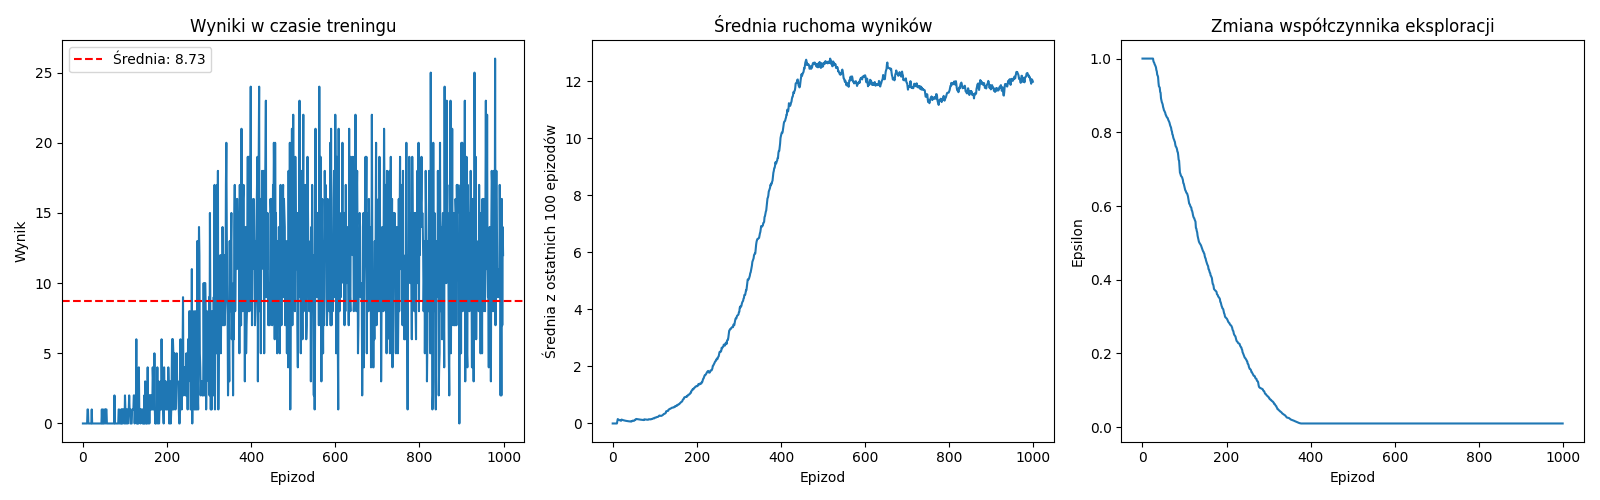
\includegraphics[width=1\linewidth]{1000gierCPU.png}
    \caption{Wyniki treningu agenta w grze Snake z użyciem CPU (1000 epizodów)}
    \label{fig:wyniki_treningu_cpu}
\end{figure}
 Parametry treningu GPU to:
\begin{itemize}
    \item Rozmiar partii: 256
    \item częstotliwość aktualizacji modelu: 2
    \item Czas treningu: 3.5 minuty
    \item najlepszy wynik: 31
    \item Wyniki dziesięciu gier testowych po wytrenowaniu: [6, 5, 6, 9, 13, 7, 21, 18, 16, 14]
    \item Średni wynik po 10 grach: 11.5
\end{itemize}

  \begin{figure}[H]
    \centering
    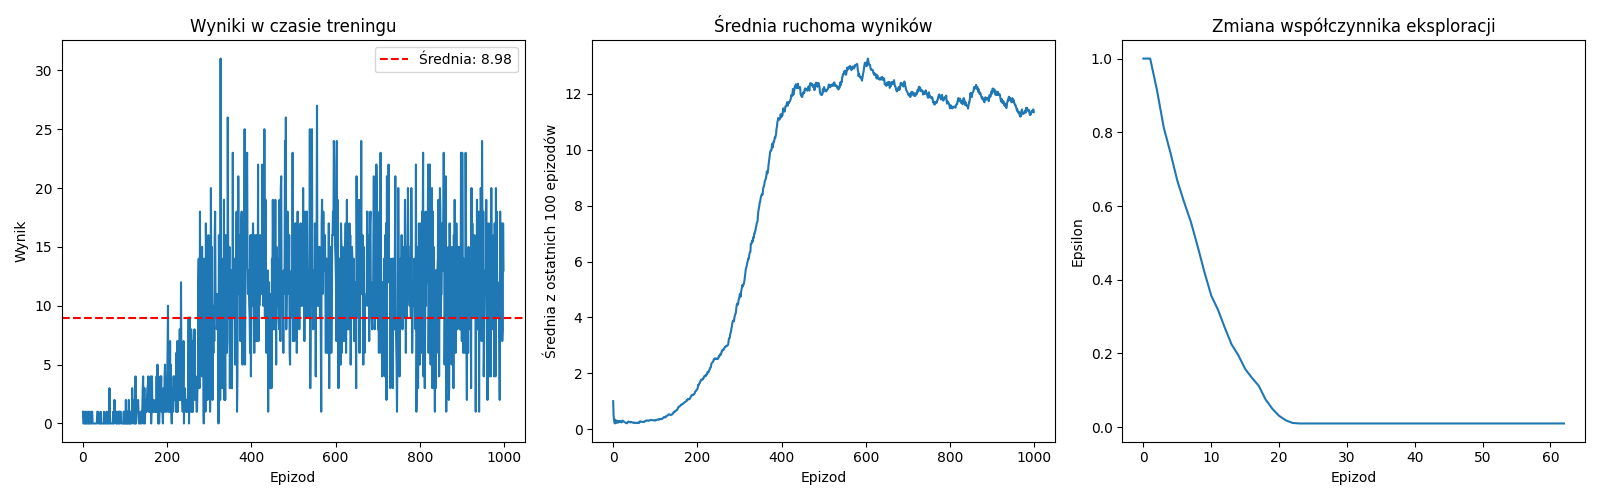
\includegraphics[width=1\linewidth]{1000gierGPU.png}
    \caption{Wyniki treningu agenta w grze Snake z użyciem GPU (1000 epizodów)}
    \label{fig:wyniki_treningu_gpu}
\end{figure}



\subsubsection{Metodologia badawcza}

Przeprowadzono eksperymentalną analizę porównawczą procesu treningu głębokiej sieci Q-learning (DQN) w kontekście implementacji agenta dla gry Snake. Eksperyment realizowano na dwóch platformach obliczeniowych: centralnej jednostce przetwarzania (CPU) oraz jednostce przetwarzania graficznego (GPU), przy zachowaniu identycznych parametrów uczenia dla obu implementacji, z wyjątkiem rozmiaru partii dostosowanego do specyfiki architektury (\(n_{batch}^{CPU} = 64\), \(n_{batch}^{GPU} = 256\)).

\subsubsection{Rezultaty eksperymentalne}


Analiza eksperymentalna wykazała istotną dysproporcję w wydajności obliczeniowej między platformami CPU i GPU, manifestującą się redukcją czasu treningu zgodnie z zależnością:

\begin{equation}
E_{czasowa} = \frac{t_{CPU}}{t_{GPU}} = \frac{45~\text{min}}{3,5~\text{min}} \approx 12,86
\end{equation}

\noindent gdzie \(E_{czasowa}\) oznacza współczynnik efektywności czasowej, \(t_{CPU}\) oraz \(t_{GPU}\) czas treningu dla odpowiednich platform.

\subsubsection{Dynamika procesu uczenia}

Zaobserwowano istotne różnice w dynamice procesu uczenia, szczególnie w odniesieniu do parametru eksploracji \(\varepsilon\) (epsilon). W implementacji GPU parametr ten osiągał wartość minimalną (\(\varepsilon_{min} = 0,1\)) znacznie szybciej, co wynika z zastosowanej techniki przetwarzania równoległego. Zbieżność parametru \(\varepsilon\) jest skorelowana z liczbą fragmentów przetwarzania równoległego:

\begin{equation}
N_{fragmentów} = \left\lceil \frac{N_{epizodów}}{N_{równoległych}} \right\rceil \approx \frac{1000}{16} \approx 63
\end{equation}

\noindent gdzie \(N_{epizodów}=1000\) oraz \(N_{równoległych}=16\) oznaczają odpowiednio liczbę epizodów treningowych oraz liczbę równolegle przetwarzanych gier.

\subsubsection{Efektywność końcowa modelu}

Analiza ilościowa wyników końcowych wskazuje na brak statystycznie istotnych różnic w efektywności agentów trenowanych na CPU i GPU:

\begin{align}
\bar{x}_{CPU} &= \bar{x}_{GPU} = 11,5 \\
\max(x_{CPU}) &= 26 \\
\max(x_{GPU}) &= 31
\end{align}

\noindent gdzie \(\bar{x}\) oznacza średnią wartość wyniku w 10 sesjach testowych, a \(\max(x)\) maksymalny uzyskany wynik.
\subsubsection{Wnioski z badania}

Przeprowadzone badania eksperymentalne potwierdzają hipotezę o niezmienności efektywności modelu względem platformy obliczeniowej przy zachowaniu identycznych parametrów algorytmu, z odpowiednim dostosowaniem parametrów zależnych od architektury. Jednocześnie wykazano znaczną przewagę GPU w aspekcie wydajności obliczeniowej, co implikuje możliwość przeprowadzenia większej liczby eksperymentów w analogicznym czasie.

\clearpage
\subsection{Porównanie wpływu wielkości okna na wyniki}

\begin{figure}[H]
    \centering
    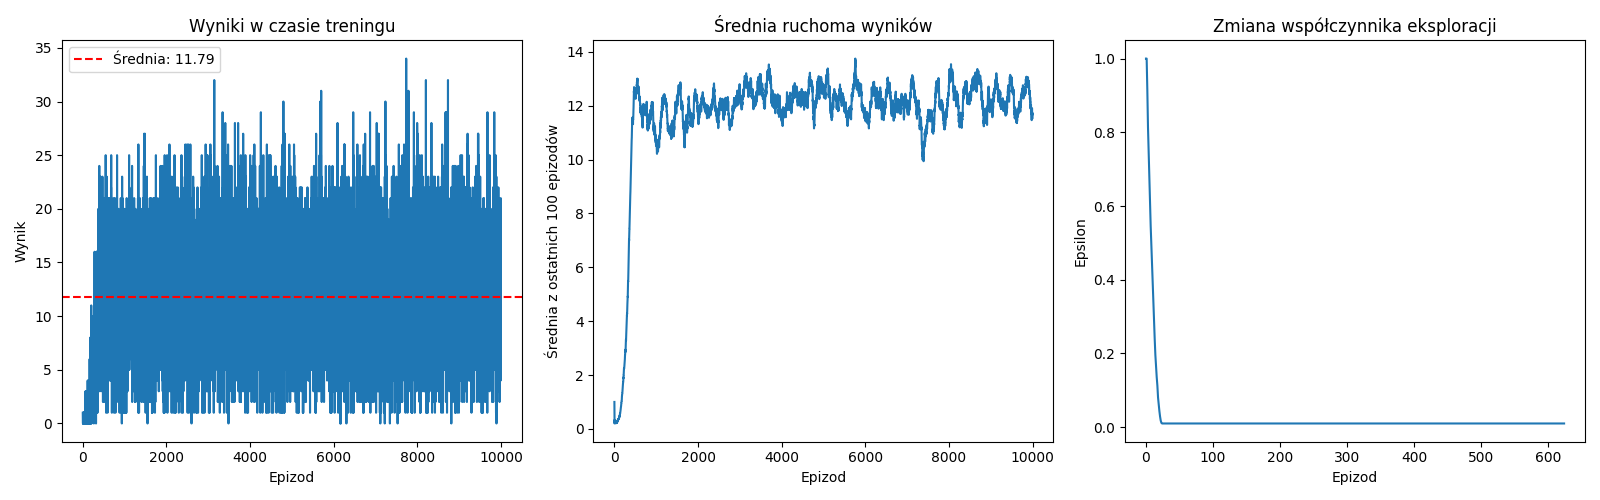
\includegraphics[width=1\linewidth]{rozdzialka320.png}
    \caption{Wyniki treningu agenta w grze Snake z użyciem rozdzielczości 320x240 pikseli (10000 epizodów)}
    \label{fig:wyniki_treningu_320}
\end{figure}

\begin{figure}[H]
    \centering
    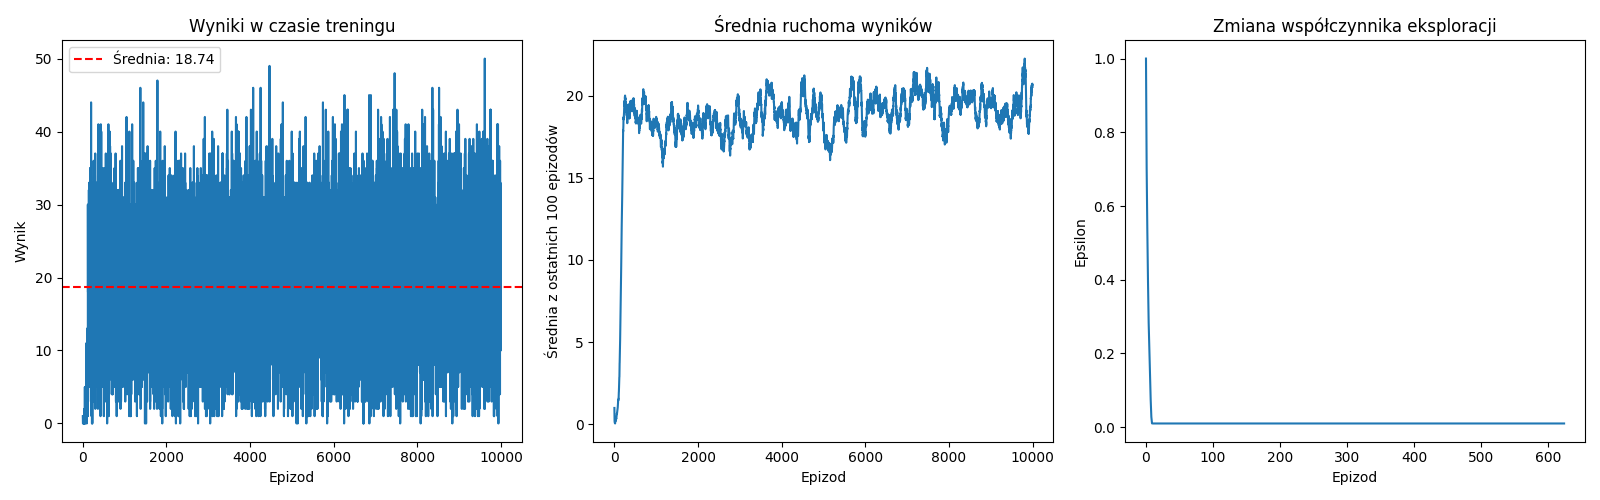
\includegraphics[width=1\linewidth]{rozdzialka640.png}
    \caption{Wyniki treningu agenta w grze Snake z użyciem rozdzielczości 640x480 (10000 epizodów)}
    \label{fig:wyniki_treningu_640}
\end{figure}

Jednym z istotnych wyzwań w projektowaniu środowisk treningowych dla algorytmów uczenia przez wzmacnianie jest precyzyjny dobór parametrów opisujących przestrzeń stanów. W ramach projektu \emph{SnakeAI} przeprowadzono serię kontrolowanych eksperymentów mających na celu ocenę wpływu rozdzielczości okna gry na jakość procesu uczenia agenta.

Analiza rezultatów wykazała, że różnica w skuteczności pomiędzy dwiema testowanymi konfiguracjami była stosunkowo niewielka. Model trenujący się w środowisku o rozdzielczości $320\times240$ pikseli osiągnął średni wynik na poziomie $11{,}79$ punktu, natomiast zwiększenie rozdzielczości do $640\times480$ pikseli przełożyło się na wzrost tej wartości do $18{,}74$ punktu. Pomimo niemal dwukrotnego powiększenia okna gry poprawa o około $60\%$ nie okazała się proporcjonalna do wzrostu rozdzielczości, co sugeruje rosnące koszty obliczeniowe przy stosunkowo niewielkich korzyściach w postaci wyższych wyników.

Wyniki te wskazują, że dalsze zwiększanie rozdzielczości środowiska może wiązać się z coraz mniejszym zwrotem z inwestycji obliczeniowej, co stanowi istotny wniosek przy optymalizacji zasobów w przedsięwzięciach wykorzystujących uczenie przez wzmocnienie.

\subsubsection{Porównanie wyników obu modeli po 10 grach testowych}
\subsubsection*{Rozdzielczość 320x240}
Wszystkie wyniki: [20, 9, 15, 9, 14, 7, 14, 12, 5, 10] \\
Średni wynik po 10 grach: 11.50

\subsubsection*{Rozdzielczość 640x480}
Wszystkie wyniki: [26, 23, 18, 20, 30, 23, 15, 21, 20, 25]\\
Średni wynik po 10 grach: 22.10 \\ 

Jednakże, w przypadku rozdzielczości 640x480 na przestrzeni mniejszej ilości próbek, agent osiągnął znacznie lepsze wyniki w testach, co sugeruje, że większa rozdzielczość może przyczynić się do lepszego zrozumienia otoczenia przez agenta, jednak dalsze próby zwiększania rozdzielczości wymagałyby o wiele lepszego sprzętu i ogromnego pokładu czasowego. Reasumując, rozdzielczość 320x240 jest wystarczająca do nauki agenta w grze Snake, a dalsze zwiększanie rozdzielczości może nie przynieść proporcjonalnych korzyści w wydajności.


\subsubsection{Porównanie wyników obu modeli po 10 grach testowych}

\paragraph{320×240}  
Wyniki indywidualne w 10 grach:  
\[
[20,\;9,\;15,\;9,\;14,\;7,\;14,\;12,\;5,\;10]
\]
Średni wynik w serii to \(11{,}50\).

\paragraph{640×480}  
Wyniki indywidualne w 10 grach:  
\[
[26,\;23,\;18,\;20,\;30,\;23,\;15,\;21,\;20,\;25]
\]
Średni wynik w serii to \(22{,}10\). \\

Chociaż agent osiągnął wyższe wyniki przy rozdzielczości 640×480, większa liczba pikseli nie przekłada się na lepsze działanie samego agenta, ponieważ w naszym podejściu sieć MLP otrzymuje wyłącznie wektor 11 binarnych cech stanu, a nie surowy obraz. Dalsze zwiększanie rozdzielczości jedynie podnosiłoby wymagania sprzętowe i czas symulacji, nie wpływając znacznie na proces uczenia. W związku z tym rozdzielczość 320×240 jest wystarczająca do efektywnej nauki agenta w grze Snake, a jej dalsze podwyższanie może nie przynieść proporcjonalnych korzyści.  



\subsection{Wpływ współczynnika uczenia na wyniki agenta}
\label{sec:experiments:learning_rate}

Aby zbadać wpływ wartości współczynnika uczenia (\emph{learning rate}) na jakość polityki agenta, przeprowadziliśmy serię eksperymentów dla trzech wartości parametru: 
\[
\alpha \in \{0.0003,\,0.003,\,0.03\}.
\]
Dla każdej wartości \textbf{lr} trenowaliśmy agenta przez 300 epizodów w identycznych warunkach i mierzyliśmy trzy statystyki końcowe:
\begin{itemize}
  \item maksymalny wynik z całego treningu,
  \item średni wynik z wszystkich epizodów,
  \item średnia z ostatnich 10 epizodów.
\end{itemize}

\begin{figure}[H]
  \centering
  \includegraphics[width=0.8\linewidth]{lr_wyniki_słupkowy.png}
  \caption{Porównanie maksymalnego, średniego oraz ostatnią dziesiątkę wyników agenta dla różnych wartości współczynnika uczenia.}
  \label{fig:lr_bar}
\end{figure}

Na ilustracji~\ref{fig:lr_bar} widać, że:
\begin{itemize}
  \item Najlepsze rezultaty (maksymalny wynik $= 42$, średnia $\approx12$, ostatnia dziesiątka $\approx13$) osiągnął agent z \(lr = 0.0003\).
  \item Dla \(lr = 0.003\) wyniki były nieco niższe (maksymalny wynik\ $= 38$, średnia $\approx10$, ostatnia dziesiątka $\approx16$) – gęstsze aktualizacje przyspieszyły naukę, ale nieznacznie obniżyły szczytowe osiągi.
  \item Najwyższa wartość \(lr = 0.03\) skutkowała najsłabszymi wynikami (maksymalny wynik \ $= 32$, średnia $\approx7$, ostatnia dziesiątka $\approx15$), co wskazuje na nadmierne wahania aktualizacji i słabszą konwergencję.
\end{itemize}

\clearpage
Dodatkowo na Rysunku~\ref{fig:lr_curve} przedstawiono krzywe zmiany średniej ruchomej wyników (okno 10 epizodów) w toku uczenia:

\begin{figure}[H]
  \centering
  \includegraphics[width=0.8\linewidth]{porównanie_lr.png}
  \caption{Średnia ruchoma wyników (okno 10 epizodów) agenta dla trzech wartości współczynnika uczenia.}
  \label{fig:lr_curve}
\end{figure}

Analiza przebiegów na Rys.~\ref{fig:lr_curve} pokazuje:
\begin{itemize}
  \item Przy \textbf{lr} \(=0.0003\) agent stopniowo i stabilnie poprawiał wyniki, osiągając najwyższy poziom w okolicach epizodu 200–250.
  \item Dla \textbf{lr} \(=.003\) tempo nauki było szybsze do epizodu \(\sim150\), ale dalej pojawiały się większe wahania i niższa wartość asymptotyczna.
  \item Zbyt duży krok \textbf{lr} \(= 0.03\)\ prowadził do niestabilnego i wolniejszego wzrostu wyników – agent często „przeskakiwał” optima.
\end{itemize}

\subsubsection{Wnioski z eksperymentu}
Dobór współczynnika uczenia jest kluczowy dla DQN. Zbyt wysoka wartość powoduje niestabilne aktualizacje i słabszą konwergencję, zaś zbyt niska spowalnia uczenie. W naszych eksperymentach optymalnym kompromisem okazało się \(\alpha=3\times10^{-4}\), co potwierdziło zarówno analiza statystyk końcowych (Rys.~\ref{fig:lr_bar}), jak i dynamika uczenia (Rys.~\ref{fig:lr_curve}).
\clearpage





\subsection{Eksperyment ze schematami nagradzania}
\label{sec:experiments:reward_schemes}

W celu zbadania wpływu różnych kształtów funkcji nagrody na zachowanie agenta DQN w grze Snake, przeprowadzono eksperymenty z pięcioma schematami nagradzania:
\begin{itemize}
  \item \textbf{default} – schemat domyślny (nagroda za jedzenie = +10, kara za śmierć = –10, +0.1 za zbliżenie, –0.1 za oddalenie),
  \item \textbf{sparse} – rzadkie nagrody (tylko +10 za jedzenie i –10 za śmierć, brak nagród i kar za zbliżenie i oddalenie),
  \item \textbf{dense} – gęstsze nagrody (nagroda za zbliżenie = +0.5, kara za oddalenie = –0.5, reszta jak w schemacie domyślnym),
  \item \textbf{food\_focus} – nacisk na jedzenie (jedzenie = +20, pozostałe parametry jak w schemacie domyślnym),
  \item \textbf{survival\_focus} – nacisk na przetrwanie (kara za śmierć = –20, reszta jak w schemacie domyślnym).
\end{itemize}

\begin{figure}[H] 
  \centering
  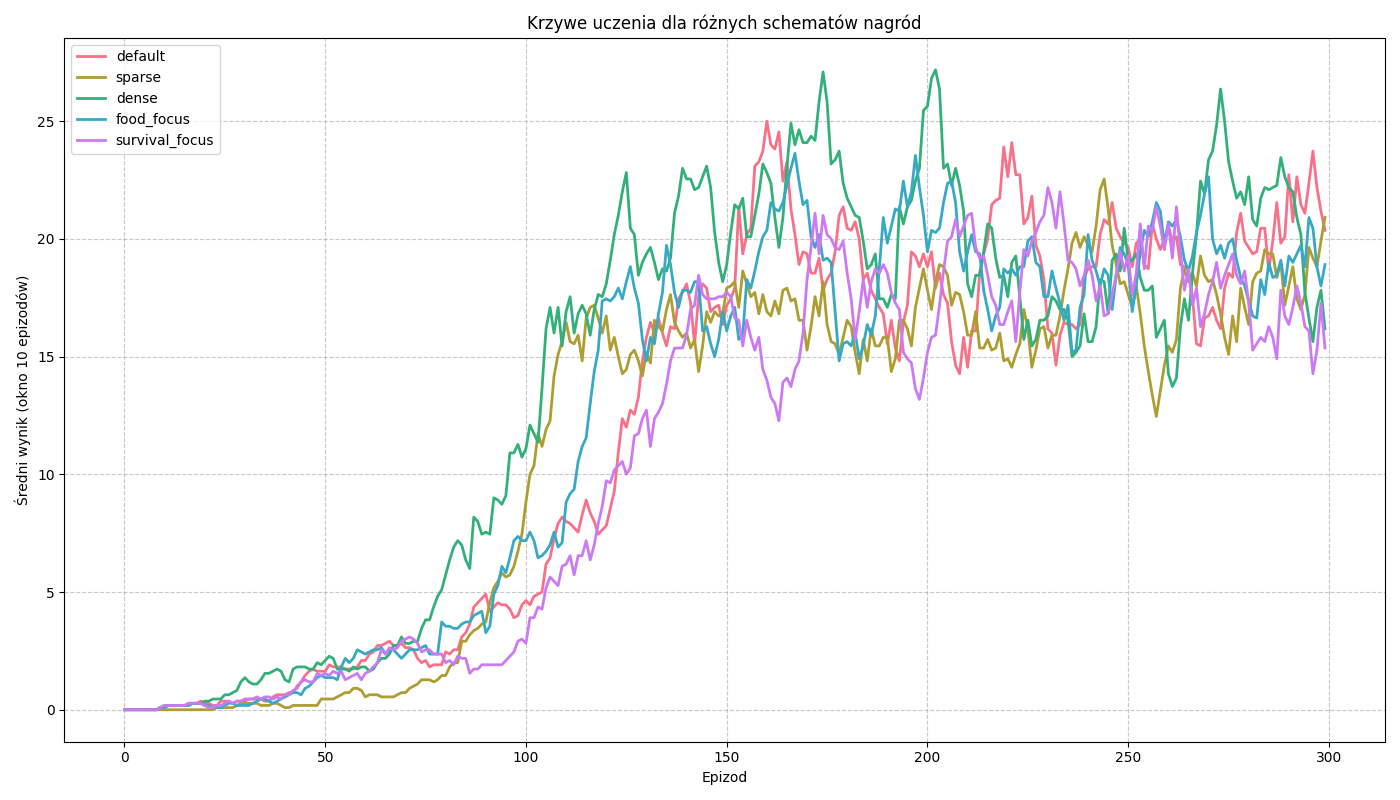
\includegraphics[width=0.85\linewidth]{krzywe_uczenia.png}
  \caption{Krzywe uczenia (średnia ruchoma z 10 epizodów) dla różnych schematów nagród.}
  \label{fig:reward_curves}
\end{figure}

Na Rysunku~\ref{fig:reward_curves} porównano tempo nauki wszystkich pięciu wariantów poprzez wizualizację średniego wyniku w oknie 10 epizodów. Widać, że:
\begin{itemize}
  \item Schemat \texttt{dense} najszybciej osiągnął wysokie wyniki (już po $\sim100$ epizodach), dzięki silnemu sygnałowi shaping.
  \item Schemat \texttt{sparse} wymagał najwięcej epizodów, by „rozgrzać” politykę, efektywniej uczył się dopiero po $\sim100$ epizodach.
  \item \texttt{food\_focus} i \texttt{survival\_focus} miały pośrednie tempo nauki, przy czym \texttt{food\_focus} szybciej podnosił wyniki w fazie wstępnej.
  \item Domyślny schemat \texttt{default} zachowywał kompromis między szybkością a stabilnością.
\end{itemize}

\begin{figure}[H] 
  \centering
  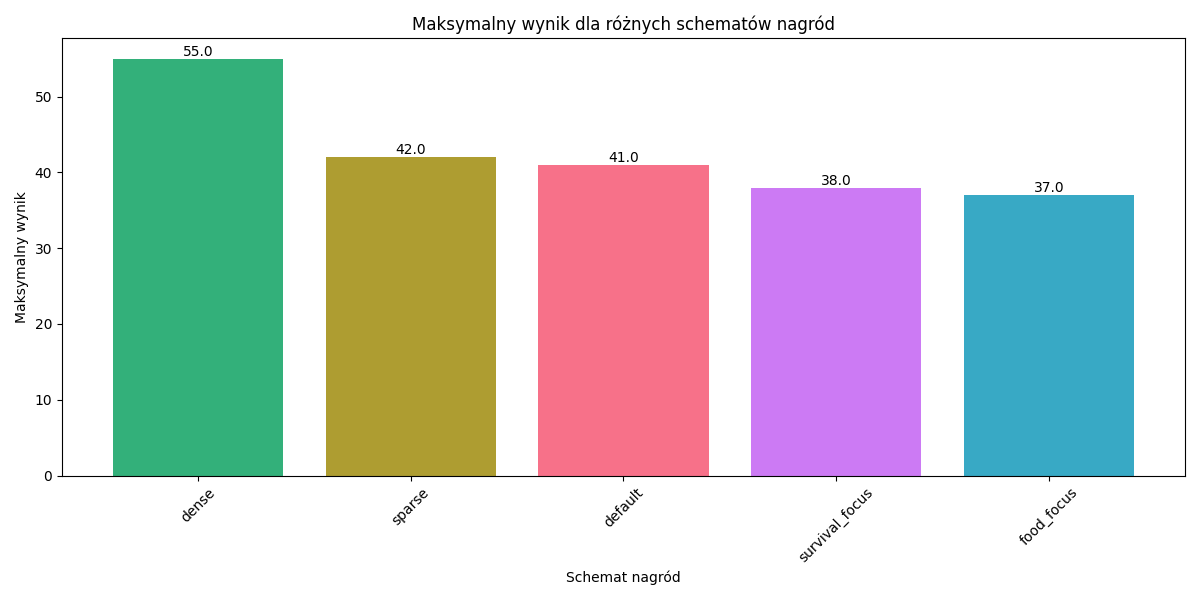
\includegraphics[width=0.85\linewidth]{maksymalne_wyniki.png}
  \caption{Maksymalne wyniki osiągnięte przez agenta w każdym schemacie nagród.}
  \label{fig:reward_max}
\end{figure}

Rysunek~\ref{fig:reward_max} przedstawia maksymalne wyniki uzyskane w trakcie całego treningu:
\begin{itemize}
  \item Najwyższy rekord (55) osiągnął schemat \texttt{dense},
  \item Kolejne miejsca zajęły \texttt{sparse} (42) i \texttt{default} (41),
  \item Najniższe maksimum (37) zanotował \texttt{food\_focus}.
\end{itemize}

\begin{figure}[H] 
  \centering
  \includegraphics[width=0.85\linewidth]{średnie_wyniki.png}
  \caption{Średni wynik (po wszystkich epizodach) dla różnych schematów nagród.}
  \label{fig:reward_mean}
\end{figure}

Na Rysunku~\ref{fig:reward_mean} pokazano średnie wyniki z pełnego przebiegu:
\begin{itemize}
  \item Najwyższą średnią (14.4) uzyskał \texttt{dense},
  \item \texttt{food\_focus} (12.8) i \texttt{default} (12.5) były na kolejnym miejscu,
  \item Najniższą średnią (11.35) odnotował \texttt{survival\_focus}.
\end{itemize}

\begin{figure}[h!] 
  \centering
  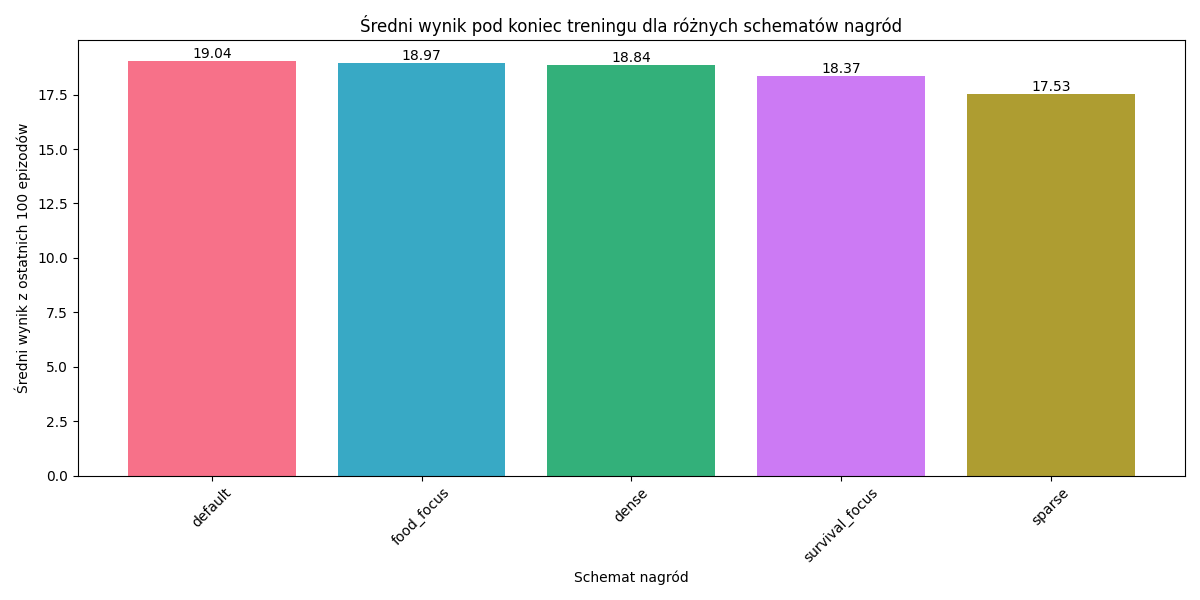
\includegraphics[width=0.85\linewidth]{końcowe_średnie.png}
  \caption{Średnie wyniki z ostatnich 100 epizodów dla różnych schematów nagród.}
  \label{fig:reward_final}
\end{figure}

Rysunek~\ref{fig:reward_final} ilustruje zachowanie agentów w fazie ustabilizowanej (ostatnie 100 epizodów):
\begin{itemize}
  \item Stabilne, wysokie wyniki (\(\approx19\)) osiągnął \texttt{default} i \texttt{food\_focus},
  \item Schemat \texttt{dense} i \texttt{survival\_focus} uzyskały porównywalne wyniki (\(\approx18.8\) i \(\approx18.4\)),
  \item \texttt{sparse} pozostał najniżej (\(\approx17.5\)), co wskazuje na większą niestabilność przy rzadszym feedbacku.
\end{itemize}

\paragraph{Wnioski z eksperymentu}
\begin{itemize}
  \item Schemat \texttt{dense} jest najlepszy do szybkiego osiągania zarówno wysokiego maksimum, jak i przyzwoitych średnich.
  \item Schemat \texttt{default} oferuje zrównoważony kompromis: dobry rekord, solidną średnią i stabilne końcowe wyniki.
  \item Schemat \texttt{sparse} wymaga znacznie więcej epizodów i wciąż pozostaje mniej stabilny w końcowej fazie.
  \item Modyfikacje wymuszające priorytet na jedzenie (\texttt{food\_focus}) lub na przeżycie (\texttt{survival\_focus}) pozwalają dostosować zachowanie agenta do konkretnych celów: agresywne zdobywanie punktów lub ostrożne przetrwanie.
\end{itemize}

Podsumowując, do końcowego projektu wybrany schemat domyślny nie okazał się być najlepszym rozwiązaniem, jednakże jego stabilność i zrównoważenie w połączeniu z innymi parametrami (np. współczynnikiem uczenia) pozwoliły na osiągnięcie dobrych wyników. Schemat \texttt{dense} okazał się być najlepszym rozwiązaniem, co pozwoli usprawnić kolejne iteracje projektu, w potrzebie o jego rozbudowę.









\clearpage
  \section{Podsumowanie i wnioski}

Przeprowadzone badania i implementacja autonomicznego agenta gry Snake z wykorzystaniem algorytmów uczenia ze wzmocnieniem pozwoliły na osiągnięcie założonych celów projektu oraz dostarczyły cennych wniosków dotyczących optymalizacji tego typu systemów.

\subsection*{Główne osiągnięcia projektu}
\begin{enumerate}
  \item Pomyślna implementacja agenta DQN zdolnego do samodzielnej nauki w grze Snake, osiągającego wyniki przewyższające losowe strategie i podstawowe heurystyki.
  \item Opracowanie hybrydowej architektury obliczeniowej łączącej zalety CPU i GPU, co znacząco przyspieszyło proces uczenia – jak wykazano w eksperymentach, nawet 12-krotnie w porównaniu do implementacji wyłącznie na CPU.
  \item Implementacja zaawansowanych technik optymalizacji, takich jak Double DQN oraz równoległa symulacja wielu instancji środowiska.
\end{enumerate}

\subsection*{Kluczowe wnioski z eksperymentów}
\begin{enumerate}
  \item \textbf{Architektura sieci neuronowej:} Oryginalna czterowarstwowa sieć (QNetwork) osiągnęła najlepsze wyniki (średni wynik 15,60) przy jednocześnie najniższej stracie (1,99). Jednowarstwowa sieć z 256 neuronami stanowi atrakcyjną alternatywę, łącząc porównywalną wydajność (średni wynik 15,00) z krótszym czasem treningu.
  \item \textbf{Platformy obliczeniowe:} Trening na GPU oferuje znaczącą przewagę w szybkości (12,86 razy szybciej niż na CPU), przy identycznej efektywności końcowego agenta. Umożliwia to przeprowadzenie większej liczby eksperymentów w krótszym czasie, co jest kluczowe w procesie optymalizacji hiperparametrów.
  \item \textbf{Rozdzielczość środowiska:} Zwiększenie rozdzielczości obrazu gry z 320×240 do 640×480 przyniosło poprawę średniego wyniku o około 60\%, jednak kosztem zwiększonych wymagań obliczeniowych. Dla dalszych badań rekomendowana jest rozdzielczość 320×240 jako optymalny kompromis między jakością reprezentacji a efektywnością obliczeń.
  \item \textbf{Współczynnik uczenia:} Optymalna wartość współczynnika uczenia wyniosła \(\alpha = 0{,}0003\). Wyższe wartości (0,003; 0,03) prowadzą do przyspieszenia początkowej fazy uczenia, ale skutkują niższą stabilnością i gorszymi wynikami maksymalnymi, co potwierdza kluczowe znaczenie tego parametru dla zbieżności algorytmu DQN.
  \item \textbf{Schematy nagradzania:} Schemat gęstych nagród (dense) okazał się najefektywniejszy, osiągając najwyższy rekord (55) oraz najwyższą średnią (14,4). Przewyższył zarówno schemat domyślny (rekord 41, średnia 12,5), jak i schematy z rzadkimi nagrodami (sparse) i z nastawieniem na przetrwanie lub zdobywanie jedzenia.
\end{enumerate}

\subsection*{Podsumowanie}

Przeprowadzone badania potwierdziły efektywność algorytmu Deep Q-Network oraz jego wariantu Double DQN w uczeniu autonomicznego agenta gry Snake. Opracowane optymalizacje, w szczególności hybrydowa architektura CPU/GPU oraz równoległa symulacja środowiska, stanowią wartościowy wkład w dziedzinę praktycznego zastosowania uczenia ze wzmocnieniem.

Najlepsze wyniki uzyskano przy zastosowaniu czterowarstwowej sieci neuronowej, współczynnika uczenia \(\alpha = 0{,}0003\) oraz gęstego schematu nagradzania (dense), co wskazuje na kluczowe znaczenie odpowiedniego doboru architektury oraz funkcji nagrody w algorytmach uczenia ze wzmocnieniem.

Przedstawione wnioski i optymalizacje mogą znaleźć zastosowanie nie tylko w kontekście gry Snake, ale również w szerszym spektrum problemów decyzyjnych wymagających uczenia sekwencyjnych strategii w złożonych środowiskach.  

\clearpage
\section{Bibliografia}  
\renewcommand{\refname}{Literatura}
\begin{thebibliography}{9}

\bibitem{RZajdelNeuron}
Zajdel R., \textit{Sztuczna inteligencja / Metody sztucznej inteligencji w sterowaniu, Laboratorium, Ćwiczenie 4: Model Neuronu},\\
\url{https://materialy.prz-rzeszow.pl/pracownik/pliki/34/%C4%86WICZENIE%2061.pdf}.

\bibitem{RZajdelMLP}
Zajdel R., \textit{Sztuczna inteligencja / Metody sztucznej inteligencji w sterowaniu, Laboratorium, Ćwiczenie 7: Sieć neuronowa jednokierunkowa wielowarstwowa},\\
\url{https://materialy.prz-rzeszow.pl/pracownik/pliki/34/ĆWICZENIE%209.pdf}.

\bibitem{mnih2015human}
Mnih V., Kavukcuoglu K., Silver D., Graves A., Antonoglou I., Wierstra D., Riedmiller M.,\\
\textit{Human-level control through deep reinforcement learning},\\
Nature.
\url{https://www.nature.com/articles/nature14236}.

\bibitem{H.vanHasselt2016}
Hado van Hasselt, Arthur Guez, David Silver, \\
\textit{Deep Reinforcement Learning with Double Q-learning},\\
\url{https://cdn.aaai.org/ojs/10295/10295-13-13823-1-2-20201228.pdf}

\bibitem{harvard}
R. Sutton, A. Barto, Reinforcement Learning: An Introduction, 2nd ed., 2018. \url{https://web.stanford.edu/class/psych209/Readings/SuttonBartoIPRLBook2ndEd.pdf}

\bibitem{PolitechnikaGdańska}
Wydział Elektroniki, Telekomunikacji i Informatyki, Politechnika Gdańska, \emph{Uczenie ze wzmocnieniem – materiały wykładowe do kursu „Metody sztucznej inteligencji w sterowaniu”}, 2017, \url{https://eti.pg.edu.pl/documents/176468/53881396/UW_MSU_2017.pdf}.

\bibitem{LeakyReLU}
Leaky ReLU, \textit{Dokumentacja}, \url{https://docs.pytorch.org/docs/stable/generated/torch.nn.LeakyReLU.html} \\

\bibitem{Pytorch}
Pytorch, \textit{Dokumentacja}, \url{https://pytorch.org/docs/stable/index.html} \\



\end{thebibliography}



\end{document}
